% \chapter{Methoden und Praktiken}

%\textit{In diesem Kapitel soll beschrieben werden, wie eine Nachvollziehbarkeit in Webanwendungen erreicht werden kann. Spezielle Methoden und Praktiken sollen vorgestellt und beleuchtet werden.}
% \textit{Hier könnte unter anderem \textbf{OpenTelemetry} betrachtet werden.}

\section{Methoden für eine bessere Nachvollziehbarkeit}
\label{sec:methoden}

Wie in \autoref{sec:nachvollziehbarkeit} zu erkennen ist bietet Nachvollziehbarkeit einen wichtigen Mehrwert für Entwickler und Betreiber von Webanwendungen, wie aber kann eine verbesserte Nachvollziehbarkeit erreicht werden? In diesem Abschnitt werden einige Methoden vorgestellt mit denen diesen Ziel erreicht werden kann.

\subsection{Fehlerberichte}

\begin{wrapfigure}[16]{r}{0.4\textwidth}
\centering
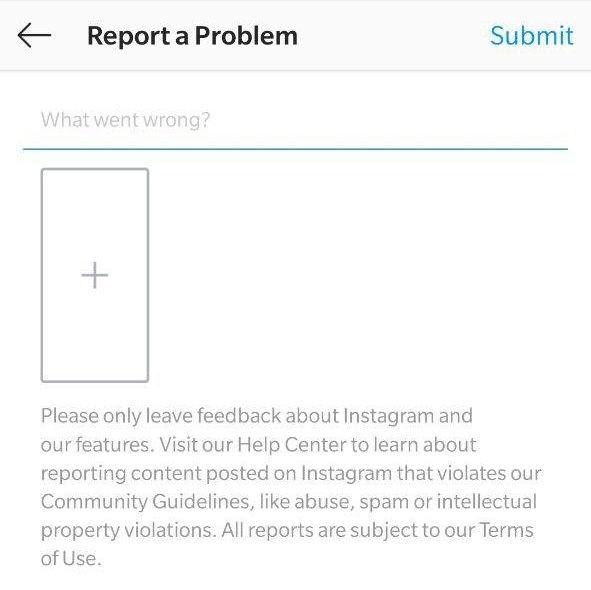
\includegraphics[width=\linewidth]{img/instagram-feedback/instagram-feedback.jpg}
\caption{Fehlerbericht in der Instagram App \cite{Instagram}}
\label{fig:instagram-bug-report}
\end{wrapfigure}

Fehlerberichte sind klassisches Mittel, um den Nutzer selbst aktiv werden zu lassen und zu erfragen, welche Aktionen er durchgeführt hat und was schiefgelaufen ist (vgl \autoref{fig:instagram-bug-report}). Hiermit können Fehler, aber auch unverständliche Workflows, aufgedeckt werden. Weiterhin können Informationen des Nutzers ermittelt werden, wie es hierzu gekommen ist und warum es ein Problem darstellt, vorausgesetzt er gibt dies an.

Konträr zu diesen Vorteilen stehen jedoch die von Bettenburg \etal \cite{WhatMakesAGoodBugReport} gesammelten Ergebnisse über die Effektivität von Fehlerberichten. Denn Nutzer meldeten Informationen und Details, die sich für die Entwickler als nicht allzu hilfreich herausstellten. Diese Diskrepanz kann u. A. dadurch erläutert werden, dass Nutzer im Regelfall kein technisches Verständnis des Systems vorweisen.

\subsection{Die Grundpfeiler der Observability}

Da Fehlerberichte somit nicht ausreichend sind, um den Entwicklern eine ausreichende Nachvollziehbarkeit zu gewährleisten, sind zusätzliche Konzepte notwendig um dies zu erreichen. Nach Sridharan \etal \cite{DistributedSystemsObservability} sowie \cite{TraefikLogsRequestTracingAndMetrics} \cite{IntrospectiveOfTheCloudManagementToolbox} \cite{MultilevelObservabilityInCloudOrchestration} existieren drei Grundpfeiler der Observability, die in ihrer Funktion einzigartig sind und sich gegenseitig ergänzen: Logs, Metriken und Traces.

\subsubsection{Logging}

%\textit{Folgende Fragen sollen zur Methode beantwortet werden}
%\begin{enumerate}
%	\item \textit{Gibt es Besonderheiten zu Logging in anderen Projekten (Backend vs. Frontend)?}
%	\item \textit{Wie können Logs an einen auswertenden Stakeholder gelangen?}
%	\item \textit{Welches Verhalten kann hiermit aufgedeckt/nachvollziehbar gemacht werden?}
%\end{enumerate}

Logging bezeichnet die systematische Protokollierung von Softwareprozessen und ihren internen Zuständen \cite{LearningToLog}. Diese erstellten Protokolle werden Logs genannt, sie helfen Betreibern und Entwicklern nach der Ausführung einer Anwendung nachvollziehen zu können, wie die genaue Verarbeitung war. Die daraus resultierende Nachvollziehbarkeit setzt jedoch voraus, dass genügend und informationsreiche Logmeldungen in die Anwendung eingebaut wurden und dass diese verstanden werden konnten \cite{LearningToLog}.

Logs stellen meist die hauptsächliche oder einzige Methode dar, wie Betreiber und Entwickler das Verhalten einer Anwendung in einer Produktivumgebung nachvollziehen können  \cite{EventLogsForTheAnalysisOfSoftwareFailures} \cite{LearningToLog}. Gerade in Problemfällen können Logs kritische Informationen bereitstellen. Bei JavaScript-basierten Webanwendungen werden jedoch selten Logs aus einer Produktivumgebung erhoben. Dies ist u. A. durch die Notwendigkeit, die Logs von einem Endnutzersystem an ein Partnersystem weiterleiten zu müssen, zu begründen, wie in \autoref{sec:logdaten} erläutert.

Logmeldungen erfolgen meist textbasiert und in einem menschenlesbaren Format. Wenn nun ein Aggregator Informationen aus einer großen Menge von Logs extrahiert, ist so ein Format hinderlich, da es nicht effizient analysiert werden kann. Um dem entgegen zu wirken, kommt Structured-Logging ins Spiel. Bei Structured-Logging \cite{StructuredAndInteroperableLogging} werden die Logmeldungen in einem vordefinierten Format erzeugt. Dieses Format kann entweder auch menschenlesbar sein oder definiert die Logmeldung bspw. als JSON-Objekt. Durch die feste Definition des Formates wird bei der Loganalyse ermöglicht, effizient die notwendigen Daten zu extrahieren.

Wird Structured-Logging eingesetzt und ein System analysiert die Protokolldaten auf enthaltene Werte, so wird ermöglicht, dass diese Protokolle nicht nur manuell einzusehen sind, sondern dass auch auf Basis dessen komplexe Datenanalysen durchgeführt werden können \cite{StructuredAndInteroperableLogging}. Mit diesen Datenanalysen lassen sich auch bei großen Datenmengen situationsrelevante Informationen entlocken \cite{StructuredLoggingCraftingUsefulMessageContent}. Weiterhin lassen sich so aus Logmeldungen auch spezielle Informationen wie Metriken extrahieren.

\subsubsection{Metriken}

Metriken sind numerische Repräsentationen von Daten, die in einer Zeitspanne aufgenommen wurden. Mithilfe von Metriken können mathematische Konzepte dazu verwendet werden, um Verständnis zu gewinnen und Vorhersagen zu treffen \cite{DistributedSystemsObservability}. Metriken sind zudem optimal für effiziente Datenbankabfragen sowie eine Langzeitspeicherung geeignet. Dies der Fall, da die Struktur der Daten einheitlich ist und sie zum Großteil lediglich numerische Werte beinhalten, was sie zudem aggregierbar macht.

\begin{wrapfigure}[10]{r}{0.35\textwidth}
\centering
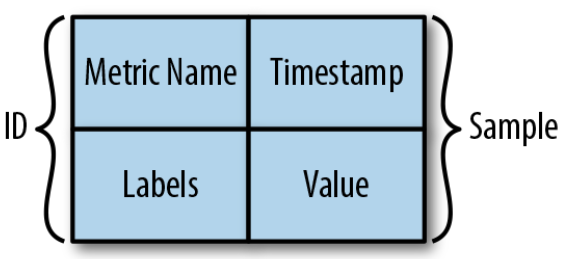
\includegraphics[width=\linewidth]{img/03_methoden/prometheus-metric-sample.png}
\caption{Struktur eines Prometheus-Metrik-Datensatzes \cite{DistributedSystemsObservability}}
\label{fig:prometheus-metric-datensatz}
\end{wrapfigure}

Beispielsweise identifiziert Prometheus \cite{Prometheus} Metriken über einen eindeutigen Namen und Schlüsselwertpaare (vgl. \autoref{fig:prometheus-metric-datensatz}) und speichert die assoziierten Daten mit einem Zeitstempel und einem Fließkommawert. Zudem können Technologien rund um die Metrikerhebung einfacher mit großen oder ansteigenden Datenaufkommen reagieren, da die Daten aggregierbar sind \cite{DistributedSystemsObservability}. Anders als z. B. bei Logsystemen, bei denen sich entweder die Auslastung bei mehr Daten erhöht oder Daten verworfen werden müssen, leiden Metriksysteme durch die Eigenschaften von Metriken selbst weniger darunter.

Durch die Kompatibilität, mathematische Konzepte auf Metriken anwenden zu können, eignen sie sich zudem dafür, eine Übersicht eines Gesamtsystems bereitzustellen und ermöglichen, so die Verfügbarkeit überprüfbar zu gestalten \cite{MultilevelObservabilityInCloudOrchestration} \cite{DistributedSystemsObservability}. Jedoch besitzen Metriken durch genau diese Eigenschaften auch Grenzen, sie können bspw. wenig aussagekräftig für das Verständnis des Verhaltens einzelner Komponenten zu einem Zeitpunkt sein. Hierbei können wiederrum Logs getrennt Aufschluss über die einzelnen Komponenten bieten. Damit die Kommunikation zwischen Komponenten oder Systemen nachvollziehbar wird, besonders aus Sicht eines einzelnen ursprünglichen Aufrufs, sind weder Logs noch Metriken ausreichend zielführend - aus diesem Grund entwickelte sich das Tracing \cite{MultilevelObservabilityInCloudOrchestration} \cite{DistributedSystemsObservability}.

\subsubsection{Tracing}
\label{sec:tracing}

Tracing beschäftigt sich mit dem Aufzeichnen von Kommunikationsflüssen in Softwaresystemen \cite{TowardsPerformanceToolingInteroperability}. Hierbei erfasst Tracing einerseits die Kommunikationsflüsse innerhalb einer Anwendung bzw. innerhalb eines Systems. Andererseits zeichnet Tracing aber auch die Kommunikationsflüsse bei verteilten Systemen auf, um diese, meist komplexen Zusammenhänge, zu veranschaulichen. Ein Tracing von verteilten Systemen nennt man \enquote{Distributed-Tracing}. Ein herstellerunabhängiger Standard, der sich aus diesem Gebiet entwickelt hat, ist OpenTracing \cite{OpenTracing}.

OpenTracing bildet diese Kommunikationsflüsse über zwei grundlegende Objekte ab: Traces und Spans. Ein Span besitzt einen Anfangs- und einen Endzeitpunkt und \textit{umspannt} meist eine Methode, bei einer Webanwendung kann dies eine Verarbeitung sein oder einen durch den Nutzer hervorgerufenen Eventfluss. Ein Span kann Kindspans beinhalten, wenn während des Lebenszyklusses weitere Spans erzeugt wurden (z. B. durch einen Methodenaufruf). Ein Trace ist eine Menge von Spans, die alle über eine einzelne logische Aktion - wie z. B. den Druck einer Taste - ausgelöst wurden oder resultieren. Ein Trace lässt sich einerseits über die kausalen Beziehungen zwischen den Spans visualisieren (vgl. \autoref{fig:otel-causal-relationship}), oder auch über die zeitliche Reihenfolge der einzelnen Spans (vgl. \autoref{fig:otel-temporal-relationship}).

Ein verteilter Trace, oftmals \enquote{Distributed-Trace} genannt, ist ein Trace, der sich aus den Spans verschiedener Systeme zusammensetzt, die miteinander kommunizieren. Hierbei werden die Traceinformationen oftmals über zusätzliche Felder bei existierenden Aufrufen propagiert, wie z. B. dem Einfügen eines Trace-Headers bei HTTP-Anfragen. Die dann an ein Tracesystem gemeldeten Spans gehen somit über die Grenzen von Anwendungen, Prozessen und Netzwerken hinaus und bilden somit einen Distributed-Trace \cite{OpenTracingSpecification}. Auf Basis von reellen Aufrufen können somit die tatsächlichen Zusammenhänge der einzelnen Systeme miteinander nachempfunden werden.

\begin{minipage}{.47\textwidth}
	\centering
	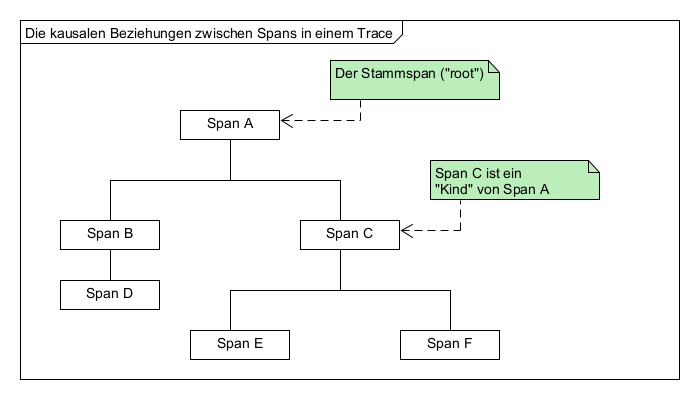
\includegraphics[width=\linewidth]{img/03_methoden/otel_causal-relationship.png}
	\captionof{figure}{Kausale Beziehung zwischen Spans. Eigene Darstellung.}
	\label{fig:otel-causal-relationship}
\end{minipage}%
\hspace{.06\textwidth}
\begin{minipage}{.47\textwidth}
	\centering
	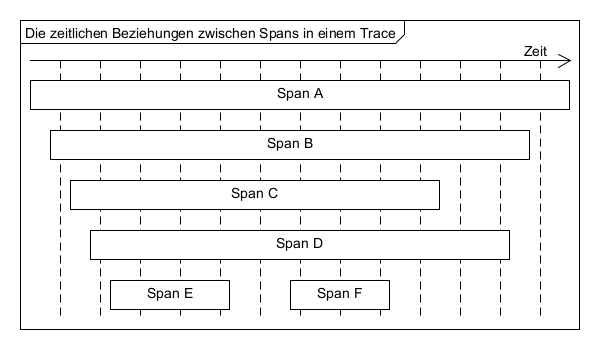
\includegraphics[width=\linewidth]{img/03_methoden/otel_temporal-relationship}
	\captionof{figure}{Zeitliche Beziehung zwischen Spans. Eigene Darstellung.}
	\label{fig:otel-temporal-relationship}
\end{minipage}

\subsection{OpenTelemetry}
\label{subsec:opentelemetry}
% \subsection{OpenTelemetry}
% \label{subsec:opentelemetry}

Es haben sich auf Basis dieser drei Grundpfeiler einige Technologien entwickelt. Jedoch sind die meisten Ansätze proprietär und nicht miteinander kompatibel, weswegen das Bedürfnis einer Standardisierung entstand. OpenTracing, OpenCensus \cite{OpenCensus} sowie OpenTelemetry \cite{OpenTelemetry} sind aus dieser Bewegung stammende Standards, die darauf abzielen herstellerunabhängige Observability-Konzepte zu definieren.

OpenTelemetry (OTel) ist ein sich derzeit\footnote{Ein erster (General-Availability-)Release der Spezifikation ist für die erste Hälfte 2021 geplant \cite{OpenTelemetryGARelease} (Stand 01.03.2021)} entwickelnder Standard, welcher als Ziel hat, das Erfassen, Weiterleiten und Verarbeiten von Tracing-, Metrik- und Logdaten\footnotemark{} herstellerunabhängig zu ermöglichen. OTel entwickelte sich aus dem Zusammenschluss der Teams hinter den beiden Standards OpenTracing und OpenCensus, die das gleiche Ziel der Vereinheitlichung, der hier existierenden Ansätze, verfolgen  \cite{UseNixDistributiveTracing}. Weiterhin versucht OTel nicht nur die bisherige Landschaft zu vereinigen, sondern definiert u. A. eine zukunftsorientierte Architektur, die aus unterschiedlichen Komponenten besteht und wie diese miteinander kommunizieren \cite{DistributedTracingInPractice}. Microsoft, Google, führende Unternehmen und Entwickler von Observability-Technologien sowie die Cloud-Native-Computing-Foundation (CNCF) arbeiten an der Entwicklung des OTel Standards \cite{DistributedTracingInPractice} \cite{OpenTelemetryCommunityMembers}.

\nomenclature[Fachbegriff]{OTel}{OpenTelemetry}
\nomenclature[Fachbegriff]{CNCF}{Cloud-Native-Computing-Foundation}
\footnotetext{Die Entwicklung einer Logging-Spezifikation ist im Gange \cite{OpenTelemetryLoggingSpecification}.}

Der OpenTelemetry-Standard definiert einige Komponenten, die jeweils spezielle Aufgabengebiete erfüllen und standardisiert mit anderen Komponenten kommunizieren. Die Komponenten werden nachfolgend näher erläutert anhand des Beispiels eines Tracing-Spans sowie der \autoref{fig:otel-components}.

\begin{itemize}
	\item \textbf{API}: Die API stellt die öffentlich sichtbare Schnittstelle der \enquote{low-level} OTel-Verarbeitung (des SDKs) dar, Verwender sind Entwickler sowie instrumentierende Bibliotheken. Mit der API kann ein Entwickler einen Trace initialisieren, darauf aufbauend einen Span erzeugen und diesen Span starten.
	
	\item \textbf{Instrumentation-Library}: Bei einer solchen Bibliothek handelt es sich um eine spezifische Anbindung der OTel-API bspw. an ein Framework (wie JAX-RS oder Angular). Teilweise erlauben solche Bibliotheken auch eine automatische Erfassung der Daten, sodass bei relevanten Methoden (wie Schnittstellaufrufen) automatisch ein Span erzeugt wird.
	
	\item \textbf{SDK}: Das SDK stellt das Herzstück der Verarbeitung bei OTel dar und pflegt u. A. die Beziehung zwischen den Spans sowie reicht diese an Verarbeitungsmethoden weiter, letztendlich werden sie an exportierende Komponenten übergeben. Der erzeugte Span wird mit seinen Kontextinformationen im SDK vorgehalten und bei Beendigung des Spans wird dieser an die angebunden Exporter übergeben.
	
	\item \textbf{Exporter}: Exporter sind spezifische Anbindungen, die Daten im OTel-Format annimmt und diese für Gegenstellen aufbereitet sowie an diese transportiert. Die Gegenstelle kann entweder eine Datensenke darstellen oder auch eine weiterverarbeitende Komponente sein. In diesem Beispiel (vgl. \autoref{fig:otel-components}) wird der Span nicht in ein anderes Format überführt, da er an einen OTel-Colletor gesendet wird.
	
	\item \textbf{Collector}: Collector sind eine OTel-Schnittstelle, um unterschiedliche OTel-Daten anzunehmen und diese an weitere Systeme mithilfe von Exportern zu überreichen. Bei dem Exporter in diesem Beispiel werden die Daten in das passende Format des Telemetry-Backends überführt.
	
	\item \textbf{Telemetry-Backend}: Ein Telemetry-Backend stellt die Datensenke der OTel-Daten dar und bietet den Entwicklern und Betreibern eine Visualisierung der gesammelten Daten. Beispiele hierfür sind z. B. Jaeger \cite{Jaeger} oder Prometheus \cite{Prometheus}.
\end{itemize}
 
\begin{figure}[H]
	\centering
	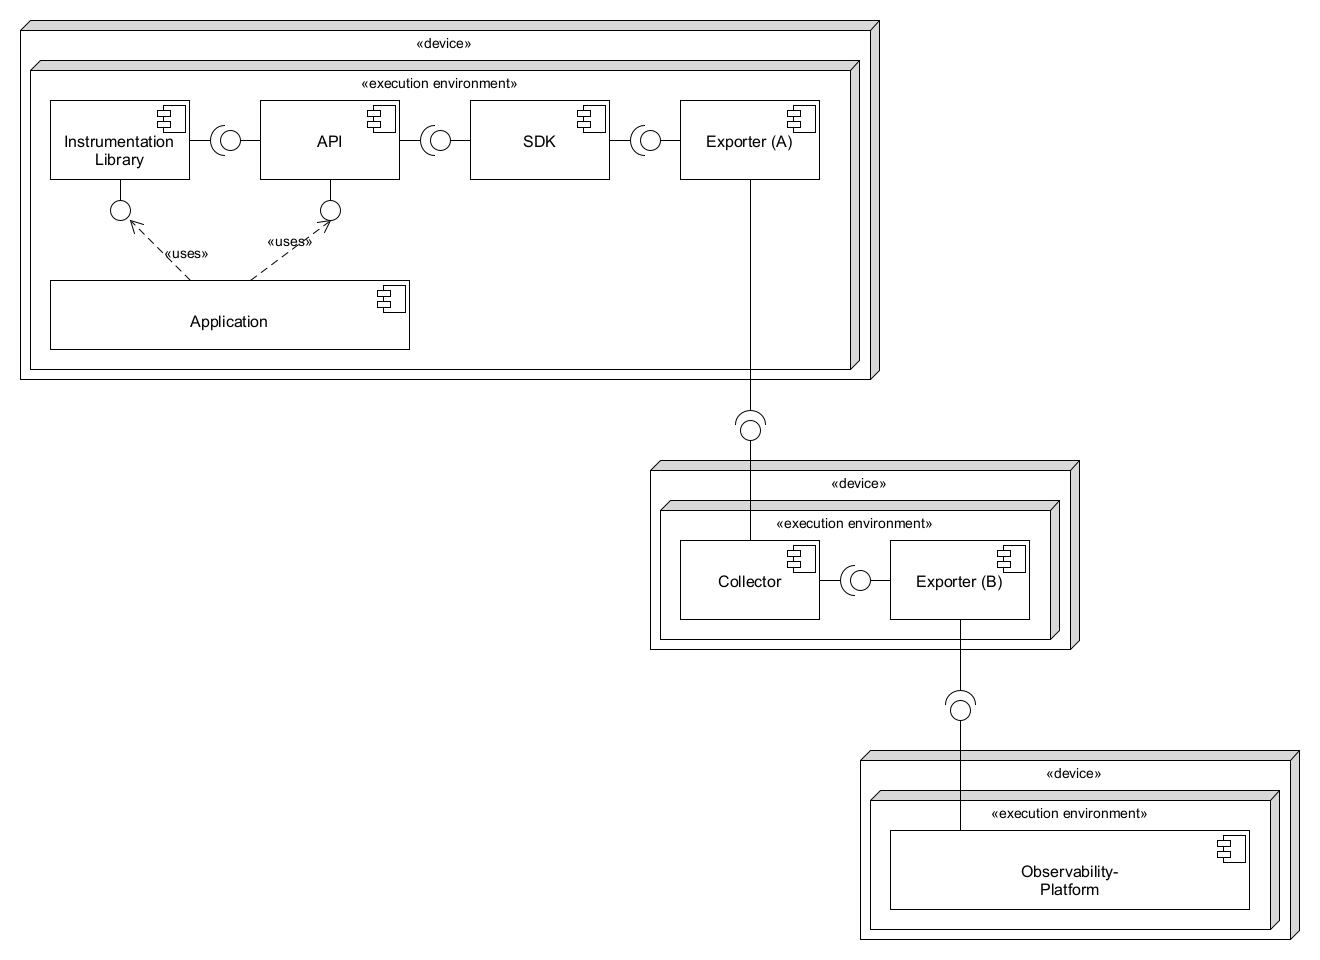
\includegraphics[width=1.00\linewidth]{img/03_methoden/otel_components.png}
	\caption{Komponenten von OpenTelemetry, eigene Darstellung auf Basis von \cite{OTelSpecification}}
	\label{fig:otel-components}
\end{figure}

OpenTelemetry legt somit ein fundiertes Konzept fest, welches die Interoperabilität der derzeit existierenden Systeme erhöhen wird, vorausgesetzt der Standard wird erfolgreich veröffentlicht und auch adaptiert.

% \section{Praktiken}

% \subsection{Fachpraxis}

\subsection{Application-Performance-Monitoring (APM)}

In der Fachpraxis haben sich über die Jahre einige Technologien entwickelt und etabliert, welche die Nachvollziehbarkeit von Anwendungsverhalten und Nutzerinteraktion ermöglichen oder verbessern. Auf Basis der zuvor vorgestellten Methoden und teils neuer Ansätze haben sich in der Wirtschaft einige Praktiken entwickelt. Eines dieser Ansätze ist das Application-Performance-Monitoring (APM, teils auch Application-Performance-Management).

APM lässt sich nicht simpel definieren, denn es existiert kein Konsens, welche Eigenschaften und Funktionalitäten ein APM umfasst. Ahmed \etal \cite{StudyingTheEffectivenessOfAPMTools}, Heger \etal \cite{APMStateOfTheArtAndChallenges}, Rabl \etal \cite{SolvingBigDataChallengesForAPM} sowie Dynatrace \cite{DynatraceAPM} definieren, dass APM eine Menge an Methoden, Techniken und Werkzeugen umfasst, die das System konstant überwachen und Aufschluss über den Zustand geben, sodass die Verfügbarkeit des Systems sichergestellt werden kann. Anders definieren dies jedoch Santos Filipe \cite{ClientSideMonitoringOfDistributedSystems}, New Relic \cite{NewRelicAPM} und Gartner \cite{GartnerMagicQuadrantForAPM}, welche APM weniger allgemeingültig definieren, sondern APM eher über explizite Teilaspekte definieren, die es erfüllen muss, damit es sich um ein konformes APM handelt. Jedoch existiert hier ebenso kein Konsens, welche expliziten Aspekte erfüllt sein müssen, damit ein Monitoring-System zu einem APM wird.

In dieser Arbeit wird auf Basis der ersten und eher allgemeingültigen Definition ein APM so definiert: APM befasst sich mit dem Beobachten eines Softwaresystems und der Gewinnung von relevanten Daten aus diesem System zur näheren Analyse, um zu ermöglichen, dass Rückschlüsse über die Gesundheit des Systems gezogen werden können und so die Verfügbarkeit sichergestellt werden kann. Um dies zu erreichen, lassen sich grob 5 Fachgebiete differenzieren, die unterschiedliche Aspekte eines Softwaresystems aufdecken \cite{ASurveyOfCloudMonitoringTools} \cite{GartnerMagicQuadrantForAPM} \cite{ResearchAndApplicationOfOperatingMonitoring}:

\begin{enumerate}
	\item Infrastruktur-Monitoring (IM)
	\item Application-and-Service-Monitoring (ASM)
	\item Real-User-Monitoring (RUM)
	\item Error-Monitoring
	\item Distributed-Tracing
\end{enumerate}

\subsubsection{Infrastructure-Monitoring (IM)}

Infrastructure-Monitoring beschäftigt sich hauptsächlich mit der Überwachung der Infrastruktur. Hierbei wird bspw. die Verfügbarkeit von Netzwerkressourcen überwacht sowie die Auslastung von Hard- und Softwareressourcen. Dieses Monitoring kann ohne Anpassungen der Software erfolgen und stellt somit ein Beispiel für Black-Box-Monitoring dar \cite{ClientSideMonitoringOfDistributedSystems}. Beispielsweise ist die Überwachung von CPU- und Speicherausnutzung eines Containers Teil von Infrastructure-Monitoring.

\subsubsection{Application-and-Service-Monitoring (ASM)}

Anders als beim System-Monitoring handelt es sich bei Application-and-Service-Monitoring (ASM, teilweise auch Application-Component-Monitoring) um White-Box-Monitoring. Genauer bedeutet dies, dass die Softwarekomponenten angepasst werden müssen, sodass innerhalb der Laufzeitumgebungen Daten gesammelt werden können. Beispielsweise werden die Antwortzeit von Schnittstellaufrufen protokolliert und systematisch überwacht. Auf Basis der Daten lassen sich u. A. Abweichungen von der Norm feststellen, von einzelnen Systemen oder vom aktuellen Gesamtsystem zu einem vorherigen Zeitpunkt.

\subsubsection{Real-User-Monitoring (RUM)}

\nomenclature[Fachbegriff]{UI}{User-Interface}

Real-User-Monitoring beschäftigt sich mit dem Mitschneiden von allen Nutzerinteraktionen und Umgebungseigenschaften einer Benutzeroberfläche \cite{IdentifyingWebPerformanceDegradations}. Um diese Daten zu ermitteln ist eine Änderung der Software für die Benutzeroberfläche notwendig, welches RUM zu einem White-Box-Monitoring macht. RUM wird jedoch nicht dazu verwendet, die Interaktionen eines einzelnen Nutzers aufzudecken, sondern Aufschluss über die gesamte Nutzerschaft der Anwendung zu erhalten. Die Daten werden oftmals gruppiert bspw. nach den Interaktionen oder auch nach Umgebungseigenschaften, wie dem Browser der Nutzer. Durch die Gruppierung lassen sich Probleme der User-Experience feststellen \cite{AConceptLatticeForRecognitionOfUserProblems}, aber auch Leistungsprobleme der Anwendung feststellen und ob diese den unterschiedlichen Umgebungen der Nutzer geschuldet sind \cite{IdentifyingWebPerformanceDegradations}.

\subsubsection{Error-Monitoring}

Das Error-Monitoring konzentriert sich auf das Erfassen und Melden von Fehlern \cite{CrashbinCrashMonitoring}. Error-Monitoring lässt sich sowohl als White-Box- sowie als Black-Box-Monitoring umsetzen, da über existierende Protokollierung bereits Fehler festgestellt werden können, jedoch kann es hierbei sinnvoll sein eine Software anzupassen, um mehr Kontextinformationen zu erfassen. Das Error-Monitoring wird oftmals eng mit einem Issue-Management verbunden, um aufgetretene Fehler und deren Behebung nachzuhalten zu machen \cite{CrashbinCrashMonitoring}.

\subsubsection{Distributed-Tracing}

Beim Distributed-Tracing handelt es sich um die fortgeschrittene Art des Tracings, welche systemübergreifend den Durchlauf von Abfragen protokolliert (vgl. \autoref{sec:tracing}). Diese Art von Monitoring gibt, anders als die anderen Arten, keine Einsicht in einzelne Komponenten, sondern veranschaulicht die resultierenden Interaktionen einer Abfrage.

\subsection{Log-Management}

Neben dem APM gibt es zudem weitere Funktionalitäten, die Technologien in der Fachpraxis vorweisen, wie z. B. das Log-Management. Log-Management umfasst die Erfassung, Speicherung, Verarbeitung und Analyse von Logdaten von Anwendungen. Neben diesen Funktionen bieten solche Werkzeuge oftmals fundierte Suchfunktionen und Visualisierungsmöglichkeiten. Um die Daten aus einer Anwendung heraus zu exportieren, gibt es meist eine Vielzahl an Integrationen für Frameworks und Logbibliotheken.

Einer der wichtigsten Punkte beim Log Management, ist der Umgang mit großen Datenmengen und die gewünschten Operationen, die Nutzer damit durchführen möchten.

\subsection{Session-Replay}

Session-Replay beschreibt das Vorgehen, eine Sitzung eines Nutzers nachzustellen, so als ob sie gerade passiert \cite{NoBoundariesExfiltrationBySessionReplayScripts}. Hierbei können einzelne Aspekte der Anwendung nachgestellt werden, bspw. der Kommunikationsablauf oder die DOM-Manipulationen. Je mehr Aspekte nachgestellt werden, desto realitätsnaher ist die Nachstellung und entsprechend hilfreich ist sie beim Nachvollziehen.

Realitätsnahes Session-Replay nimmt somit eine enorme Datenmenge für jede Nutzersitzung auf und benötigt besonders bei Browsern eine effiziente Kommunikation, um die UX nicht negativ zu beeinflussen.

\begin{wrapfigure}[10]{r}{0.40\textwidth}
\centering
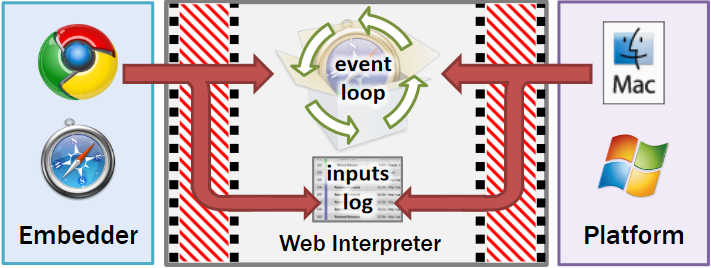
\includegraphics[width=\linewidth]{img/03_methoden/timelapse_figure5.png}
\caption{Mitschneiden von DOM-Events, Abb. aus \cite{TimelapsePaper}}
\label{fig:timelapse_figure5}
\end{wrapfigure}

Bereits 2013 entwickelten Burg \etal \cite{TimelapsePaper} mit \enquote{Timelapse} ein Framework, um Benutzersitzungen bei Webanwendungen aufzunehmen und wiederzugeben. Timelapse unterscheidet sich zu gängigen Session-Replay-Ansätzen dahingehend, dass die Wiedergabe keine vereinfachte Nachstellung der Anwendung ist. Stattdessen wird die JavaScript-Eventloop abgekapselt und es werden die Aufrufe von und zu der Eventloop mitgeschnitten (vgl. \autoref{fig:timelapse_figure5}).

\begin{wrapfigure}[10]{r}{0.40\textwidth}
\centering
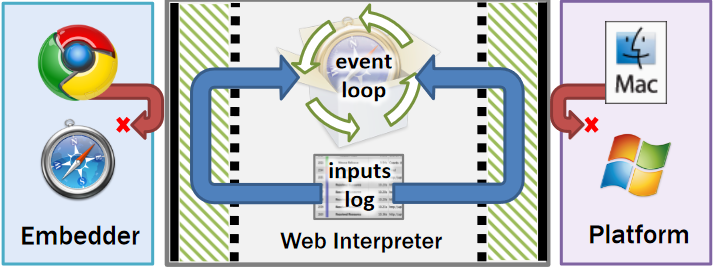
\includegraphics[width=\linewidth]{img/03_methoden/timelapse_figure6.png}
\caption{Abspielen von DOM-Events, Abb. aus \cite{TimelapsePaper}}
\label{fig:timelapse_figure6}
\end{wrapfigure}

Beim Abspielen werden die Aufrufe dann in derselben Reihenfolge an die Eventloop übergeben (vgl. \autoref{fig:timelapse_figure6}). Dies bedeutet es ist ein exaktes wiederholtes Ausführen in derselben Umgebung möglich und dies ermöglicht eine detaillierte Nachvollziehbarkeit des Anwendungsverhaltens. Leider wird für diesen Ansatz eine gepatchte Version von WebKit vorausgesetzt, somit wird auch Zugriff auf das Endnutzersystem benötigt. Aus diesem Grund und weil es sehr mehr als 5 Jahren nicht mehr gepflegt wird\footnote{Timelapse GitHub Repo \url{https://github.com/burg/replay-staging/}}, ist es ungeeignet für die hier angestrebte Lösung. Die vorgestellten Konzepte stellen jedoch nützliche Kernprinzipien für das Session Replay im Allgemeinen dar.

\subsection{OpenTelemetry}
\label{subsec:opentelemetry}

Neben diesen Praktiken haben sich in der Wirtschaft einige Standards entwickelt, um die Vorgehensweisen zu vereinheitlichen und miteinander kompatibel zu machen. Einer dieser Standards ist OpenTelemetry \cite{OpenTelemetry}.

OpenTelemetry (OTel) ist ein sich derzeit\footnote{Ein erster (General-Availability-)Release der Spezifikation ist für die erste Hälfte 2021 geplant \cite{OpenTelemetryGARelease}.} entwickelnder Standard, welcher als Ziel hat, dass das erfassen, weiterleiten und verarbeiten von  Tracing-, Metrik- und Logdaten\footnotemark{} herstellerunabhängig ermöglicht wird. OTel entwickelte sich aus dem Zusammenschluss der Teams hinter den beiden Standards OpenTracing und OpenCensus \cite{OpenCensus}, die das gleiche Ziel der Vereinheitlichung, der hier existierenden Ansätze, verfolgen  \cite{UseNixDistributiveTracing}. Weiterhin versucht OTel nicht nur die bisherige Landschaft zu vereinigen, sondern definiert bspw. eine zukunftsorientierte Architektur aus unterschiedlichen Komponenten und wie diese miteinander kommunizieren \cite{DistributedTracingInPractice}. Microsoft, Google, die Cloud-Native-Computing-Foundation (CNCF) sowie führende Unternehmen und Entwickler von Observability-Technologien arbeiten an der Voranschreite des OTel Standards \cite{DistributedTracingInPractice} \cite{OpenTelemetryCommunityMembers}.

\nomenclature[Fachbegriff]{OTel}{OpenTelemetry}
\nomenclature[Fachbegriff]{CNCF}{Cloud-Native-Computing-Foundation}
\footnotetext{Die Entwicklung einer Logging-Spezifikation ist im Gange \cite{OpenTelemetryLoggingSpecification}.}

 \textit{\color{red} TODO: OpenTelemetry detaillierter beschreiben}

%OpenTelemetry (OTel) \cite{OpenTelemetry} ist ein sich derzeit\footnote{Ein erster (General-Availability-)Release der Spezifikation ist für Q1 2021 geplant \cite{OpenTelemetryGARelease}.} entwickelnder herstellerunabhängiger Standard, um Tracing-, Metrik- und Logdaten\footnotemark{} zu erfassen, zu verarbeiten, zu analysieren und zu visualisieren. OTel fasst die beiden Standards OpenTracing und OpenCensus \cite{OpenCensus} zusammen und hat sich als Ziel gesetzt diese zu erweitern \cite{UseNixDistributiveTracing}. Hinter dem Standard stehen u. A. die Cloud Native Computing Foundation (CNCF), Google, Microsoft, und führende Hersteller von Tracing- und Monitoring-Lösungen.
%
%Ziel ist es, dass Entwickler Tools und Werkzeuge benutzen können, ohne erneut hochspezifische Anbindungen schreiben und konfigurieren zu müssen. Stattdessen definiert der Standard Komponenten, die spezielle Aufgabengebiete haben und mit einer allgemeinen API anzusprechen sind. Die technische Infrastruktur einer auf OTel basierenden Lösung ist in \autoref{fig:otel-unified-collection} zu sehen. Im groben definiert OTel folgende Komponenten: API, SDK, Exporter, Collector und Backend (vgl. \autoref{fig:otel-components}).
%
%\nomenclature[Fachbegriff]{OTel}{OpenTelemetry}
%\nomenclature[Fachbegriff]{CNCF}{Cloud Native Computing Foundation}
%\footnotetext{Eine Entwicklung einer Definition zu Logging ist im Gange \cite{OpenTelemetryLoggingSpecification}.}
%
%\begin{figure}[H]
%	\centering
%	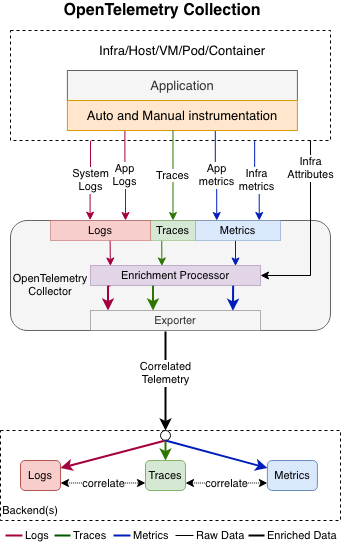
\includegraphics[width=\linewidth]{img/03_methoden/otel_unified-collection_2.png}
%	\caption{Schaubild einer Lösung auf Basis von OTel \cite{OpenTelemetryUnifiedCollection}}
%	\label{fig:otel-unified-collection}
%\end{figure}
%
%\begin{figure}[H]
%	\centering
%	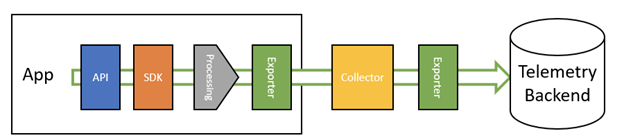
\includegraphics[width=0.75\linewidth]{img/03_methoden/dynatrace_otel-components.png}
%	\caption{OTel Komponenten \cite{DynatraceOTelComponents}}
%	\label{fig:otel-components}
%\end{figure}

\section{Werkzeuge und Technologien}
\label{sec:werkzeuge-und-technologien}
%\section{Werkzeuge und Technologien}
%\label{sec:werkzeuge-und-technologien}

%\textit{Basierend auf dem Grundwissen über die Methoden und Praktiken, soll nun der Stand der Technik erörtert werden. Hierbei sollen Werkzeuge und Technologien und ihre Ansätze hervorgehoben werden und mit Hilfe welcher Methoden sie welches Ziel erreichen.}
%
%\textit{Wie in der Zielsetzung definiert sollen hier zwei bis drei Technologien näher vorgestellt werden.}
%
%\textit{Weiterhin könnte beleuchtet werden, wie ähnliche Herausforderungen bei anderen „Fat-Client“-Lösungen (also nicht SPAs) angegangen werden, und kann man hier vielleicht etwas lernen oder übertragen (und wenn nicht, warum nicht)?}

Um die gewünschte Lösung, den Proof-of-Concept, zu erstellen, muss zuvor der Stand der Technik erörtert werden. In diesem Abschnitt wird ein Überblick über aktuelle Technologien gegeben. Die vorgestellten Technologien werden kategorisiert und nach zuvor definierten Kriterien bewertet. Daraus ergibt sich eine Auswahl, der für den Proof-of-Concept in Frage kommenden Technologien.

\subsection{Recherche}

Um relevante und aktuelle Technologien zu ermitteln, wurde neben verfügbarer Literatur auch auf etablierte Plattformen bei der Gegenüberstellung von Technologien gesetzt. Dabei wurden Gartner\footnote{Gartner ist ein global agierendes Forschungs- und Beratungsunternehmen im Bereich der IT \cite{GartnerDefinition}} und StackShare\footnote{StackShare (\url{https://stackshare.io}) ist eine Vergleichsseite für Entwicklerwerkzeuge und Technologien, die auf Basis von Nutzereingaben Vergleiche erzeugt \cite{StackshareDefinition}} eingesetzt. Die identifizierten Technologien werden im nachfolgenden Abschnitt vorgestellt. 

Mithilfe von Gartners \enquote{Magic Quadrant for APM} \cite{GartnerMagicQuadrantForAPM} konnte festgestellt werden, dass folgende Werkzeuge zu den führenden Technologien in der Kategorie angehören: \textit{AppDynamics} \cite{AppDynamics}, \textit{Dynatrace} (ehemals ruxit) \cite{Dynatrace}, \textit{New Relic} \cite{NewRelic}, \textit{Broadcom DX APM} \cite{BroadcomDXAPM}, \textit{Splunk APM} \cite{SplunkAPM} sowie \textit{Datadog} \cite{Datadog}. Bestätigt werden einige dieser Technologien in der Bewertung bei StackShare \cite{StackShareAPM}. Hier sind insbesondere New Relic und Datadog zu erwähnen oft sowie  die Application Insights \cite{AzureApplicationInsights} des \textit{Azure Monitors} von Microsoft.

In der Literatur finden sich auch Vergleiche und Empfehlungen, so fanden z. B. Mart{\'i}nez \etal \cite{ComparisonOfE2ETestingToolsForMicroservices} in ihrer Evaluierung von Werkzeugen bei der Unterstützung von E2E-Tests, dass die beiden OpenSource-Technologien \textit{Jaeger} \cite{Jaeger} und \textit{Zipkin} \cite{Zipkin} aktiv dabei helfen können Fehlerszenarien in Microservice-Architekturen besser nachzuvollziehen. Weiterhin beschrieben Li \etal \cite{ServiceMeshChallengesStateOfTheArt}, wie mit \textit{Prometheus} \cite{Prometheus}, Jaeger, Zipkin und \textit{Fluentd} \cite{Fluentd} eine Datenanalyse von Microservices ermöglicht werden kann. Hinzukommend beschreiben Picoreti \etal \cite{MultilevelObservabilityInCloudOrchestration} eine Observability-Architektur, die auf Fluentd, Prometheus und \textit{Zipkin} basiert.

Bei StackShares Gegenüberstellung von Error-Monitoring-Produkten \cite{StackShareExceptionMonitoring} stechen drei Technologie heraus: \textit{Sentry} \cite{Sentry}, \textit{TrackJS} \cite{TrackJS} sowie \textit{Rollbar} \cite{Rollbar}. Die zwei erst genannten waren zudem auch bei der Gegenüberstellung der Monitoring-Lösungen \cite{StackShareMonitoring} gelistet.

StackShare bezeichnet Session-Replay als \enquote{User-Feedback-as-a-Service}. Hierbei \cite{StackShareUserFeedbackAsAService} lassen sich ebenfalls drei etablierte Produkte identifizieren: \textit{Inspectlet} \cite{Inspectlet}, \textit{FullStory} \cite{FullStory} und \textit{LogRocket} \cite{LogRocket}. Während Inspectlet und FullStory hauptsächlich auf die Nachvollziehbarkeit von User-Experience abzielen, konzentriert sich LogRocket auf technische Informationen, die für Entwickler von Bedeutung sind \cite{Webalyt}. Gartner bietet zudem eine Übersicht \cite{GartnerWebAndMobileAppAnalytics} über Produkte im \enquote{Web and Mobile App Analytics Market} an, in der sich \textit{Google Analytics} \cite{GoogleAnalytics}, \textit{Adobe Analytics} \cite{AdobeAnalytics} sowie LogRocket auf den obersten Positionen befinden.

\subsection{Übersicht}

In der \autoref{tab:technologie-uebersicht} werden nachfolgend die gefundenen Technologien näher veranschaulicht. Auf Basis der Produktbeschreibungen der Hersteller wird untersucht, welche Funktionalität die jew. Technologie vorweisen kann. Genauer werden folgende, zuvor identifizierte, Funktionalitäten unterschieden und den zugeordnet: IM, ASM, RUM, Error-Monitoring, Log-Management, (Distributed-)Tracing sowie Session-Replay. Um den Funktionsumfang zur jew. Funktionalität anzugeben, werden folgende 4 Schlüssel verwendet:

\begin{enumerate}
	\item \texttt{ja}: Die Funktionalität ist vorhanden und der Funktionsumfang entspricht der Definition.
	\item \texttt{ja(*)}: Die Funktionalität ist vorhanden, aber sie ist nicht so umfangreich wie bei anderen Technologien.
	\item \texttt{eingeschränkt}: Die Funktionalität ist nur unter bestimmten Voraussetzungen vorhanden oder ist nur teilweise implementiert.
	\item \textit{keine Angabe}: Die Funktionalität ist nicht vorhanden.
\end{enumerate}

\hvFloat[rotAngle=90,nonFloat=true,capWidth=w]%
{table}%
{
\begin{tabular}{|p{2.25cm}|p{1.5cm}|p{2.0cm}|p{3.0cm}|p{3.0cm}|p{1.5cm}|p{2.5cm}|}
\hline
Technologie & APM & RUM & Error-Mo\-ni\-tor\-ing & Log-Management & Tracing & Session-Replay \\
\hline
Adobe Analytics &  & gruppiert & teils &  &  &  \\
\hline
AppDynamics & ja & gruppiert & ja &  & ja &  \\
\hline
Broadcom DX APM & ja &  & teils & ja & ja &  \\
\hline
DataDog & ja & gruppiert & ja & ja & ja &  \\
\hline
Dynatrace & ja & gruppiert & ja & ja & ja &  \\
\hline
Elastic Stack & möglich & möglich & möglich & ja &  &  \\
\hline
Fluentd &  &  &  & ja &  &  \\
\hline
FullStory &  & ja & teils &  &  & ja \\
\hline
Google Analytics &  & gruppiert & teils &  &  &  \\
\hline
Graylog &  &  &  & ja &  &  \\
\hline
Inspectlet &  & ja & teils &  &  & ja \\
\hline
Jaeger &  &  &  &  & ja &  \\
\hline
LogRocket &  & ja & ja & teils &  & ja \\
\hline
New Relic & ja & gruppiert & ja & ja & ja &  \\
\hline
Papertrail &  &  &  & ja &  &  \\
\hline
\end{tabular}
}
{Übersicht der untersuchten Technologien, Teil 1}
{tab:technologie-uebersicht-teil1}

\hvFloat[rotAngle=90,nonFloat=true,capWidth=w]%
{table}%
{
\begin{tabular}{|p{2.25cm}|p{1.5cm}|p{2.0cm}|p{3.0cm}|p{3.0cm}|p{1.5cm}|p{2.5cm}|}
\hline
Technologie & APM & RUM & Error-Mo\-ni\-tor\-ing & Log-Management & Tracing & Session-Replay \\
\hline
Prometheus & ja &  &  &  &  &  \\
\hline
Rollbar &  & bei \mbox{Fehlern} & ja &  &  & teils \\
\hline
Sentry &  & bei \mbox{Fehlern} & ja &  &  &  \\
\hline
Splunk APM (SignalFX) & ja &  & ja &  & ja &  \\
\hline
Splunk \mbox{Enterprise} & möglich & möglich & möglich & ja &  &  \\
\hline
TrackJS &  & bei \mbox{Fehlern} & ja &  &  &  \\
\hline
Zipkin &  &  &  &  & ja &  \\
\hline
\end{tabular}
}
{Übersicht der untersuchten Technologien, Teil 2}
{tab:technologie-uebersicht-teil2}

\subsection{Kategorisierung}

Um die Veranschaulichung übersichtlicher zu gestalten, werden die Technologien auf Basis gemeinsamer Funktionalitäten kategorisiert. Auf Basis der evaluierten Funktionalitäten ergaben sich 6 Kategorien, in die die Technologien eingeordnet werden können. Diese Kategorien werden folgend erläutert:

\pagebreak

\begin{enumerate}
	\item APM-Plattformen
	\par Zu APM-Plattformen gehören allen voran Technologien, bei denen das Application-and-Service-Monitoring sowie das Infrastructure-Monitoring Kernfunktionalitäten darstellen. Bis auf ein Werkzeug begrenzen sich keine APM-Plattform nur auf diese beiden Aspekte, sondern können meist mehrere andere Funktionalitäten vorweisen. Am häufigsten sind Aspekte des Error-Monitorings, des Log-Managements sowie eines Distributed-Tracings vorzufinden. Neben technischen Aspekten bilden viele dieser Tools mithilfe von ASM und RUM auch Einsichten in die geschäftliche Leistung der Anwendung. Auf Basis von RUM wird teils Nutzerverhalten gruppiert visualisiert, um die Nutzerschaft besser verstehen zu können - eine Ansicht einer einzelnen Nutzersitzung wie beim Session-Replay ist jedoch nicht Teil dessen.
	
	\item Log-Plattformen
	\par Als Log-Plattformen werden alle Technologien bezeichnet, die eine Verarbeitung von Logdaten als ihre Kernfunktionalität verstehen. Nahezu alle hier angesiedelten Werkzeuge sind in der Lage Entwicklern und Betreibern eine detaillierte Analyse der Logdaten zu ermöglichen. Weiterhin steht oftmals die Funktionalität zur Verfügung diese Daten auch visuell Darstellungen zu können. Auf Basis der analytischen Funktionalitäten können zudem Aspekte von IM, ASM, RUM oder Error-Monitoring nachgestellt werden. Neben diesen Funktionalitäten steht aber auch ein effizientes Persistenzkonzept im Vordergrund, damit mit den enormen Datenmengen aus unterschiedlichen Systemen umgegangen werden kann \cite{TowardsAutomatedLogParsingForLargeScale}.
	
	\item Distributed-Tracing-Systeme
	\par Hiermit werden jene Technologien beschrieben, die ein Distributed-Tracing ermöglichen. Effiziente Architektur stehen oftmals im Vordergrund, welche explizit auf die enormen Datenmengen angepasst ist, die beim Distributed-Tracing anfallen können \cite{DapperInfrastructure}.
	
	\item Error-Tracking
	\par Die Kategorie Error-Tracking zeichnet sich dadurch aus, dass Technologien die Erhebung und Visualisierung von Fehlerdaten als ihre Kernfunktionalität verstehen. Weiterhin besitzen viele dieser Werkzeuge ein detailliertes Issue-Management, mit dem sich Teams organisieren können, um Fehler zu beheben und Arbeiten nachzuhalten.
	
	\item Session-Replay-Dienste
	\par Die Technologien der Kategorie Session-Replay zeichnen Nutzersitzungen auf und stellen diese Betreibern und Entwicklern in nachgestellter Videoform bereit. Hierbei lässt sich eine geschäftliche und eine technische Repräsentation unterscheiden. Bei ersterem werden Nutzersitzungen teils gruppiert und als Heatmaps dargestellt, bei letzterem werden detaillierte technische Informationen mitgeschnitten und dargestellt \cite{Webalyt}.
	
	\item Web-Analytics
	\par Die letzte Kategorie beschäftigt sich mit Web-Analytics-Technologien. Diese befassen sich mit der Evaluierung der Performance einer Webanwendung, sei es im geschäftlichen oder auch im technischen Sinne \cite{APracticalEvaluationOfWebAnalytics} \cite{WebAnalyticsAnHourADay}. Allgemeiner lässt sich anhand der Charakteristika sagen, dass Web-Analytics eine sehr spezifische Untermenge von APM-Plattformen darstellt.
	
\end{enumerate}

In der \autoref{tab:technologie-kategorisierung} werden die Technologien gruppiert nach ihrer Kategorie dargestellt. Da nicht alle Kategorien gleich hilfreich für die hier angestrebte Lösung sind, findet im \autoref{subsec:technologie-vorauswahl} eine Vorauswahl statt, welche Funktionskategorien näher betrachtet werden sollen.

\begingroup
\centering
\setlength{\LTleft}{-20cm plus -1fill}
\setlength{\LTright}{\LTleft}
\begin{longtable}{|p{4.10cm}|p{0.90cm}|p{0.90cm}|p{1.9cm}|p{1.75cm}|p{1.5cm}|p{1.4cm}|p{1.3cm}|}
\hline
Technologie & IM & ASM & RUM & Error-Montoring & Log-Mgmt. & Tracing & Session-Replay \\
\endhead
\hline
\hline
\multicolumn{8}{|l|}{APM-Plattformen} \\
\hline
AppDynamics & ja & ja & ja(*) & ja & eingeschr. & ja &  \\
\hline
Dynatrace & ja & ja & ja(*) & ja & ja & ja &  \\
\hline
New Relic & ja & ja & ja(*) & ja & ja & ja &  \\
\hline
Broadcom DX APM & ja & ja &  & teils & ja & ja &  \\
\hline
Splunk APM (SignalFX) & ja & ja &  & ja &  & ja &  \\
\hline
DataDog & ja & ja & ja(*) & ja & ja & ja &  \\
\hline
Azure Monitor & ja & ja &  & ja & ja & ja &  \\
\hline
Prometheus & ja & ja &  &  &  &  &  \\
\hline
\hline
\multicolumn{8}{|l|}{Log-Plattformen} \\
\hline
Papertrail & ja(*) & ja(*) & ja(*) & ja(*) & ja &  &  \\
\hline
Elastic Stack & ja(*) & ja(*) & ja(*) & ja(*) & ja &  &  \\
\hline
Fluentd &  &  &  &  & eingeschr. &  &  \\
\hline
Splunk \mbox{Enterprise} & ja(*) & ja(*) & ja(*) & ja(*) & ja &  &  \\
\hline
Graylog & ja(*) & ja(*) & ja(*) & ja(*) & ja &  &  \\
\hline
\hline
\multicolumn{8}{|l|}{Distributed-Tracing-Systeme} \\
\hline
Jaeger &  &  &  &  &  & ja &  \\
\hline
Zipkin &  &  &  &  &  & ja &  \\
\hline
\hline
\multicolumn{8}{|l|}{Error-Tracking} \\
\hline
Sentry &  &  & ja(*) & ja &  &  &  \\
\hline
TrackJS &  &  & ja(*) & ja &  &  &  \\
\hline
Rollbar &  &  & ja(*) & ja &  &  &  \\
\hline
Airbrake & ja & ja &  & ja &  &  &  \\
\hline
Bugsnag &  &  &  & ja &  &  &  \\
\hline
Raygun & ja & ja & ja(*) & ja &  &  &  \\
\hline
\hline
\multicolumn{8}{|l|}{Session-Replay-Dienste} \\
\hline
Inspectlet &  &  & ja & teils &  &  & ja \\
\hline
FullStory &  &  & ja & teils &  &  & ja \\
\hline
LogRocket &  &  & ja & ja &  &  & ja \\
\hline
\hline
\multicolumn{8}{|l|}{Web-Analytics} \\
\hline
Google Analytics & eing. & eing. & ja(*) & eingeschr. &  &  &  \\
\hline
Adobe Analytics & eing. & eing. & ja(*) & eingeschr. &  &  &  \\
\hline
\caption{Kategorisierung der untersuchten Technologien}
\label{tab:technologie-kategorisierung}
\end{longtable}
\endgroup


\subsection{Vorauswahl}
\label{subsec:technologie-vorauswahl}

Wie zuvor beschrieben eignen sich nicht alle Funktionskategorien teils mehr teils weniger für die, in dieser Arbeit angestrebte Lösung: Ein Proof-of-Concept, welches die Nachvollziehbarkeit einer Webanwendung von Anwendungsverhalten und Nutzerinteraktionen für \textbf{Betreiber und Entwickler} verbessert.

APM-Plattformen bieten durch ihr IM und ASM aufschlussreiche Einsichten in die Leistung und Verfügbarkeit einer Anwendung, helfen aber nicht oder kaum bei der Aufdeckung von einzelnen Problemen. Sie bieten hilfreiche Informationen aus wirtschaftlicher und operativer Sicht, bieten aber technische Informationen. Ein weiterer Grund gegen die Nutzung von Werkzeugen des Application-Performance-Monitorings ist die hier existierende Marktmacht von proprietären Lösungen. Die proprietären Ansätze zeichnen sich durch vorgefertigte Lösungen aus, die aber unflexibel in den Anpassungsmöglichkeiten sind. Um diese Diskrepanz näher zu untersuchen wurden New Relic und Dynatrace evaluiert. Hierbei konnte festgestellt werden, dass die bereitgestellten Informationen, aus Sicht eines Entwicklern, nicht ausreichend Aufschluss boten. So fehlte einedetaillierte Einsicht in einzelne Fehlerszenarien oder auch Nutzersitzungen. Stattdessen wurden gruppierte Informationen bereitgestellt, die die grobe \enquote{Gesundheit} des Systems widerspiegeln. Aus diesen Gründen, gerade aufgrund der divergierenden Zielgruppen, werden APM-Plattformen nicht näher betrachtet.

Aus einem ähnlichen Grund, wird die Kategorie Web-Analytics ebenso nicht näher behandelt. Werkzeuge im Web-Analytics-Bereich legen den Fokus sehr stark auf Überprüfung von wirtschaftlichen und operativen Eigenschaften, nicht jedoch den in dieser Arbeit erwünschten Zielen. Die übrig gebliebenen Kategorien werden im nächsten Unterabschnitt näher betrachtet und kriteriengeleitet bewertet.

\subsection{Kriterien}

Um für den Proof-of-Concept passende Technologien zu identifizieren, werden diese auf Basis verschiedener Kriterien bewertet. Diese Bewertung stützt sich auf öffentlich verfügbare Informationen, die die Hersteller der jeweiligen Technologie selber veröffentlicht haben. Die Kriterien werden folgend näher beschrieben.

\begin{enumerate}
	\item Kostenfrei
	\par Mit dem Kriterium \enquote{Kostenfrei} soll bewertet werden, ob eine kostenfreie Variante dieser Technologie existiert. Existiert eine kostenfreie Variante, wird \texttt{ja} angegeben und ansonsten \texttt{nein}. Existiert jedoch eine kostenfreie Version, die entweder von den Funktionalitäten oder der zeitlichen Nutzung beschränkt ist, wird diese mit \texttt{f. beschränkt} bzw. \texttt{z. beschränkt} angegeben.

	\item Support für Webanwendungen
	\par Bewertet, ob eine Unterstützung für das Senden von Daten von Webanwendungen existiert. Dies kann in der Form einer Anbindung (bsw. ein Agent\footnotemark{}) oder einer Schnittstelle sein. Ist eine Schnittstelle vorhanden, die aber nicht direkt aus einem Browserkontext ansprechbar ist, so ist diese Technologie mit \texttt{möglich} zu bewerten. Ist jedoch keine Schnittstelle vorhanden, die das Senden von eigenen Daten ermöglicht, so ist die Technologie mit \texttt{nein} zu bewerten.
		\footnotetext{Ein Agent ist eine Bibliothek, die die jeweiligen Daten (wie Klicks, Ladezeiten für Ressourcen und DOM-Events, usw.), eigenständig sammelt und an ein Partnersystem übertragt \cite{SolvingBigDataChallengesForAPM}}

	\item OnPremise und SaaS
	\par Mit diesen zwei Kriterien soll bewertet werden, wie diese Technologie eingesetzt werden kann. Ist sie in einer eigenen Infrastruktur aufsetzbar, also \enquote{On-Premise}, oder existiert die Technologie als buchbarer Dienst z. B. in der Cloud, also als Software-as-a-Service (SaaS).

	\item Standardisierung
	\par Setzt die jeweilige Technologie auf etablierte Standards, wie OpenTracing bei Distributed-Tracing? Falls nicht, sind einzelne Komponenten (z. B. zur Instrumentalisierung) quelloffen oder öffentlich spezifiziert, sodass diese ausgetauscht oder angepasst werden können.

	\item Multifunktional
	\par Mit dem Kriterium \enquote{Multifunktional} wird bewertet, ob eine Technologie neben der Kernfunktionalität auch weitere Funktionalitäten aufweist. Eine Technologie ist multifunktional, wenn sie min. zwei nicht nah verwandte Funktionalitäten nahezu vollständig besitzt (\texttt{ja} oder \texttt{ja(*)}). Nah verwandt sind hierbei IM und ASM.

	\item Zielgruppe
	\par Es ist einzuordnen, für welche Zielgruppen die Technologien einen Mehrwert bietet. Es werden folgende Zielgruppen differenziert: \texttt{Projektmanager}, \texttt{Fachabteilung} und \texttt{Entwickler}.
	
\end{enumerate}

Auf Basis dieser Kriterien werden nachfolgend die Technologien bewertet. Anschließend erfolgt für jede Kategorie eine Auswahl.

\subsection{Bewertung und Auswahl}
\label{subsec:bewertung-und-auswahl}

In der Kategorie \enquote{Log-Plattformen} findet sich auf Basis der Bewertung wenig Varianz zwischen den Technologien (vgl. \autoref{tab:technologie-bewertung-log-plattformen}), lediglich Fluentd sticht hervor. Dies ist dadurch erklärbar, dass Fluentd kein vollständiges Log-Management darstellt, sondern es sich um einen Logaggregator handelt \cite{FluentdAggregator}. Somit ist Fluentd nur als verwandte Technologie anzusehen und fällt somit als Präferenz aus. Der Elastic-Stack eignet sich durch die hohe Flexiblität und der Komponente Logstash auch dazu, Log-Management mit ihr zu betreiben  \cite{ThreatIdentificationFromAccessLogsUsingElasticStack} \cite{DesignLogManagementSystem}. Papertrail, Splunk sowie Graylog lassen sich als klassiche Log-Management-Werkzeuge verstehen, da sie speziell auf diese Funktionskategorie angepasst sind. Graylog sowie der Elastic-Stack sind quelloffen, aber auch als SaaS verfügbar. Bei einem gewünschten OnPremise Einsatz kann lediglich nur Papertrail nicht eingesetzt werden, denn dies wird nicht unterstüzt. Letztendlich lässt sich sagen, dass keine dieser vier Technologien ausschließende Eigenschaften besitzt, sondern allesamt für die in dieser Arbeit angestrebte Lösung geeignet sind.

Letztendlich wurde sich für \textbf{Splunk} entschieden, u. A. weil es beim Kunden bereits im Einsatz ist. Wie aber zuvor erwähnt, eignen sich die anderen Technologien ähnlich gut und eine erneute Auswahl mit anderen situationsbedingten Kriterien könnte variieren.

\begin{table}[H]%
\centering
\addtolength{\leftskip}{-2cm}
\addtolength{\rightskip}{-2cm}
\begin{tabular}{|p{3.05cm}|p{1.8cm}|p{1.7cm}|p{1.2cm}|p{1.3cm}|p{1.7cm}|p{1.3cm}|p{2.6cm}|}
\hline
Technologie & Kostenfrei & Support f. Webanw. & On \mbox{Premise} & SaaS & Standard. & Multif. & Zielgruppe \\
\hline
Papertrail & f. begrenzt & eingeschr. & nein & ja & nein & ja & Fachabteilung, Entwickler \\
\hline
Elastic Stack & ja & eingeschr. & ja & ja & eingeschr. & ja & Fachabteilung, Entwickler \\
\hline
Fluentd & ja & eingeschr. & ja & ja & eingeschr. & nein & Entwickler \\
\hline
Splunk \mbox{Enterprise} & f. begrenzt & eingeschr. & ja & ja & nein & ja & Fachabteilung, Entwickler \\
\hline
Graylog & ja & eingeschr. & ja & ja & eingeschr. & ja & Entwickler \\
\hline
\end{tabular}
\caption{Bewertung der Technologien der Kategorie \enquote{Log-Plattformen}}
\label{tab:technologie-bewertung-log-plattformen}
\end{table}


Im Gebiet der Distributed-Tracing-Systeme gibt es auch nur wenige oberflächliche Unterschiede (vgl. \autoref{tab:technologie-bewertung-distributed-tracing-systeme}). Sowohl Jaeger als auch Zipkin sind quelloffen und werden weitflächig eingesetzt \cite{AnalysisOfDistributedTracingSystemsEffectOnPerformance}. Jaeger scheint für neue Projekten attraktiver zu sein und findet dort mehr Einsatz, wie in StackShares Gegenüberstellung zu sehen ist \cite{StackShareJaegerVsZipkin}. Teilweise ist dies erklärbar durch die Ergebnisse, die Mart{\'i}nez \etal \cite{ComparisonOfE2ETestingToolsForMicroservices} herausfanden: Jaeger zeigt mehr hilfreiche Informationen an und kann diese schneller bereitstellen als Zipkin. Zudem entwickelt Jaeger aktiv eine Unterstützung des neuen OpenTelemetry-Standards \cite{JaegerOpenTelemetry}, bei Zipkin findet sich keine vergleichbare Entwicklung. Aus diesen Gründen ist \textbf{Jaeger} hierbei das Werkzeug der Wahl.

\begin{table}[H]%
\centering
\addtolength{\leftskip}{-2cm}
\addtolength{\rightskip}{-2cm}
\begin{tabular}{|p{3.05cm}|p{1.8cm}|p{1.7cm}|p{1.2cm}|p{1.3cm}|p{1.7cm}|p{1.3cm}|p{2.6cm}|}
\hline
Technologie & Kostenfrei & Support f. Webanw. & On \mbox{Premise} & SaaS & Standard. & Multif. & Zielgruppe \\
\hline
Jaeger & ja & eingeschr. & ja & nein & ja & nein & Entwickler \\
\hline
Zipkin & ja & eingeschr. & ja & nein & eingeschr. & nein & Entwickler \\
\hline
\end{tabular}
\caption{Bewertung der Technologien der Kategorie \enquote{Distributed-Tracing-Systeme}}
\label{tab:technologie-bewertung-distributed-tracing-systeme}
\end{table}


Die Auswahl in der Kategorie \enquote{Error-Tracking} ist etwas diverser (vgl. \autoref{tab:technologie-bewertung-error-tracking}), denn hier weisen manche Technologien Funktionalitäten auf, die sonst in dem Gebiet fremd sind. Bespielweise bieten Airbrake und Raygun neben einem Error-Monitoring zudem Aspekte eines APM, sodass die Anwendung/das System auch im Normalbetrieb überprüft werden kann. Diese APM-Funktionalitäten sind jedoch nicht so ausgereift, wie bei spezialisierten APM-Lösungen. Airbrake und Raygun sind lediglich als SaaS-Produkte, währenddessen Sentry, Rollbar und Bugsnag auch als OnPremise-Lösung verfügbar sind. Sentry ist zudem quelloffen auf GitHub \cite{GitHub} veröffentlicht\footnote{Sentry GitHub Repo: \url{https://github.com/getsentry/sentry}} und entwickelt dort mit der Community an dem Produkt weiter. Weiterhin ist Sentry das einzige identifizierte Werkzeug, welches eine nicht zeitlich begrenzte Version der SaaS-Lösung zur Verfügung stellt. Eine aussagekräftige Entscheidung kann jedoch nicht getroffen werden, da alle Werkzeuge des Error-Monitoring die gewünschten Anforderungen ausreichend erfüllen. Dennoch wird sich an dieser Stelle für \textbf{Sentry} entschieden, auf Basis der zuvor nahe gelegten Gründe.

\begin{table}[H]%
\centering
\addtolength{\leftskip}{-2cm}
\addtolength{\rightskip}{-2cm}
\begin{tabular}{|p{3.05cm}|p{1.8cm}|p{1.7cm}|p{1.2cm}|p{1.3cm}|p{1.7cm}|p{1.3cm}|p{2.6cm}|}
\hline
Technologie & Kostenfrei & Support f. Webanw. & On \mbox{Premise} & SaaS & Standard. & Multif. & Zielgruppe \\
\hline
Sentry & f. begrenzt & ja & ja & ja & eingeschr. & nein & Fachabteilung, Entwickler \\
\hline
TrackJS & z. und f. begrenzt & ja & nein & ja & nein & nein & Fachabteilung, Entwickler \\
\hline
Rollbar & z. und f. begrenzt & ja & ja & ja & nein & nein & Fachabteilung, Entwickler \\
\hline
Airbrake & z. und f. begrenzt & ja & nein & ja & nein & ja & Fachabteilung, Entwickler \\
\hline
Bugsnag & z. und f. begrenzt & ja & ja & ja & eingeschr. & nein & Fachabteilung, Entwickler \\
\hline
Raygun & z. und f. begrenzt & ja & nein & ja & nein & ja & Fachabteilung, Entwickler \\
\hline
\end{tabular}
\caption{Bewertung der Technologien der Kategorie \enquote{Error-Tracking}}
\label{tab:technologie-bewertung-error-tracking}
\end{table}


In der Beschreibung zur Kategorie \enquote{Session-Replay} wurde erwähnt, dass einige dieser Werkzeuge eine eher geschäfts- und andere eher eine entwicklerorientierte Session-Replay-Funktionalität vorweisen (vgl. \autoref{tab:technologie-bewertung-session-replay-dienste}). Genauer ist FullStory fast ausschließlich für das Nachvollziehen von User-Experience konzipiert, währenddessen LogRocket sehr detaillierte und sehr technische Informationen liefert \cite{Webalyt}. Inspectlet lässt sich als Mischung dieser beiden Sichten verstehen, bietet aber z. B. nicht alle Informationen an, die LogRocket darstellt  \cite{Webalyt}. Da die hier angestrebte Lösung auf Betreiber und insbesondere Entwickler abzielt, fiel die Wahl auf \textbf{LogRocket}.

\begin{table}[H]%
\centering
\addtolength{\leftskip}{-2cm}
\addtolength{\rightskip}{-2cm}
\begin{tabular}{|p{3.05cm}|p{1.8cm}|p{1.7cm}|p{1.2cm}|p{1.3cm}|p{1.7cm}|p{1.3cm}|p{2.6cm}|}
\hline
Technologie & Kostenfrei & Support f. Webanw. & On \mbox{Premise} & SaaS & Standard. & Multif. & Zielgruppe \\
\hline
Inspectlet & f. begrenzt & ja & nein & ja & nein & nein & Projektmanager, Fachabteilung, Entwickler \\
\hline
FullStory & f. begrenzt & ja & nein & ja & nein & nein & Projektmanager, Fachabteilung, Entwickler \\
\hline
LogRocket & f. begrenzt & ja & ja & ja & nein & nein & Fachabteilung, Entwickler \\
\hline
\end{tabular}
\caption{Bewertung der Technologien der Kategorie \enquote{Session-Replay-Dienste}}
\label{tab:technologie-bewertung-session-replay-dienste}
\end{table}


\subsection{Vorstellung der Technologien}

\subsubsection{Splunk}
\label{subsec:splunk}

Splunk bietet neben seiner akquirierten APM-Lösung (ehem. SignalFX) eine Log-Plattform an: Splunk Enterprise (nachfolgend einfach Splunk genannt). Dies stellt das Kernprodukt von Splunk dar und ist eine der führenden Plattformen auf dem Markt \cite{ThreatIdentificationFromAccessLogsUsingElasticStack}. Diese Lösung wird als OnPremise sowie auch als SaaS angeboten, was ein flexibles Deployment erlaubt.

Splunk bietet keine JavaScript-Bibliotheken, die das Senden von Daten an den Dienst vereinfachen - es steht jedoch mit dem HTTP Event Collector (HEC) \cite{SplunkHEC} eine Schnittstelle zur Verfügung, die eine Übermittlung von eigenen Logdaten ermöglicht. Der HEC ist standardmäßig nicht aus einem Browserkontext her verwendbar, da er mit ablehnenden CORS-Headern antwortet. Grund hierfür ist, dass der HEC nicht für dieses Szenario konzipiert wurde. Um dies zu umgehen, wurde ein Proxydienst eingerichtet, der die Daten des Frontends entgegennimmt, diese anreichert und dann an Splunk weiterleitet.

Auf Basis dieser Implementierung konnten alle Loginformationen eingesehen werden, sowie Fehlerdaten, welche zusätzlich an Splunk gemeldet wurden. Innerhalb von Splunk können mit der eigenen Search Processing Language (SPL) \cite{SplunkSPL} Abfragen durchgeführt werden (vgl. \autoref{fig:splunk_search-processing-language}). Mit dieser Sprache lassen sich, ähnlich wie bei SQL, einzelne Werte oder Listen abrufen aber auch neue komplexe Strukturen durch Unterabfragen generieren \cite{SplunkSQLtoSPL}.

\begin{figure}[H]
	\centering
	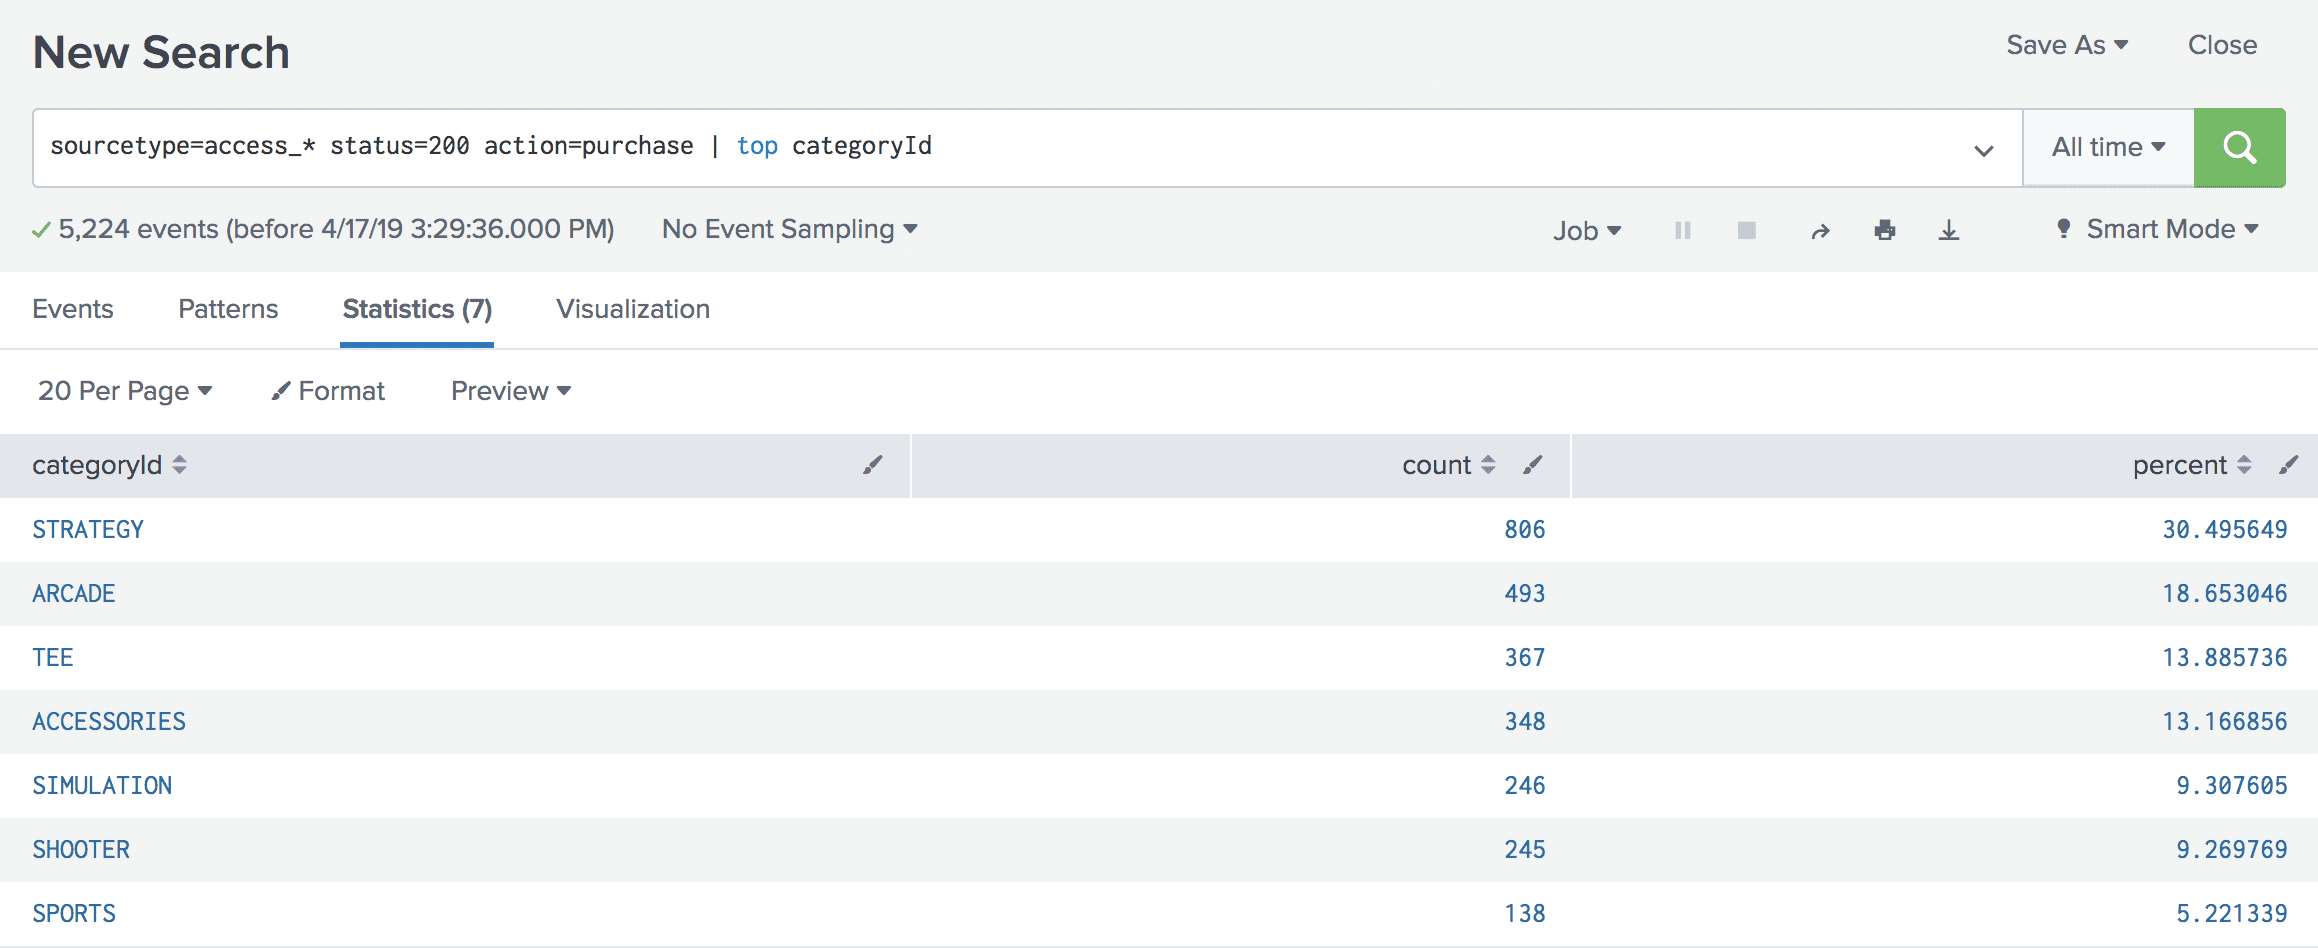
\includegraphics[width=\linewidth]{img/03_methoden/splunk_search-processing-language.png}
	\caption{Abfragebeispiel in Splunk aus \cite{SplunkSPL}}
	\label{fig:splunk_search-processing-language}
\end{figure}

\subsubsection{Jaeger}
\label{subsec:jaeger}

Jaeger wurde 2017 als ein OpenSource-Projekt der CNCF gestartet \cite{Jaeger}. Es ist ein System für verteiltes Tracing und bietet Funktionalitäten zur Datensammlung, --verarbeitung, und --speicherung bis hin zur Visualisierung. Jaeger unterstützt und implementiert den Standard OpenTracing, unterstützt aber auch Datenformate anderer Hersteller (wie z. B. Zipkin \cite{Zipkin}). Eine Unterstützung des OpenTelemetry-Standards ist derzeit in der Entwicklung. Darüber hinaus kann Jaeger genutzt werden, um Metriken nach Prometheus \cite{Prometheus} zu exportieren, einem weiteren CNCF-Projekt zur Speicherung und Visualisierung von Daten.

\begin{wrapfigure}[12]{r}{0.47\textwidth}
\centering
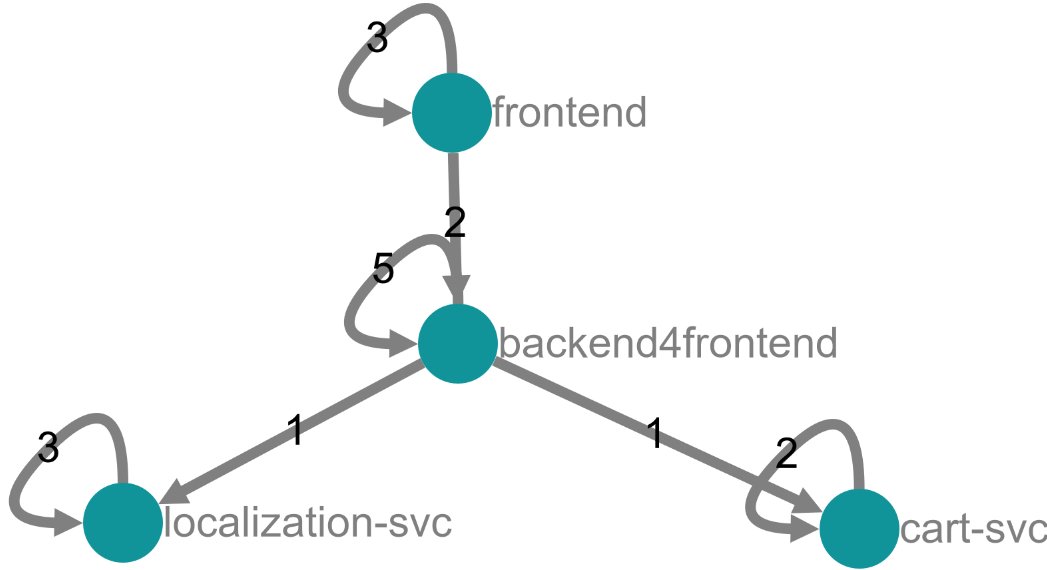
\includegraphics[width=\linewidth]{img/03_methoden/jaeger_dependency-graph.png}
\caption{Dienst-Abhängigkeits-Graph. Quelle: Eigene Darstellung}
\label{fig:jaeger-ui_dependency-graph}
\end{wrapfigure}

Jaeger spezialisiert sich auf Tracing und bietet hierfür eine skalierbare Infrastruktur zur Speicherung und Analyse der Daten. Die Traces werden als angereicherte Trace-Gantt-Diagramme dargestellt, wie in \autoref{fig:jaeger-ui_trace-detail-view} zu sehen ist. Hierbei werden sowohl hierarchische als auch zeitliche Beziehungen visualisiert. Wie bei OpenTracing und OpenTelemetry besteht ein Trace aus mehreren Spans, welche meist eine Methode umschließen. Zu den einzelnen Spans lassen sich weitere Informationen, wie bspw. Logmeldungen oder Kontextinformationen, anzeigen.

Anhand der Traces generiert Jaeger zudem automatisch eine Netzwerk-Topology, anhand der die Beziehungen zwischen Diensten nachvollzogen werden können (vgl. \autoref{fig:jaeger-ui_dependency-graph}).

\begin{figure}[H]
	\centering
	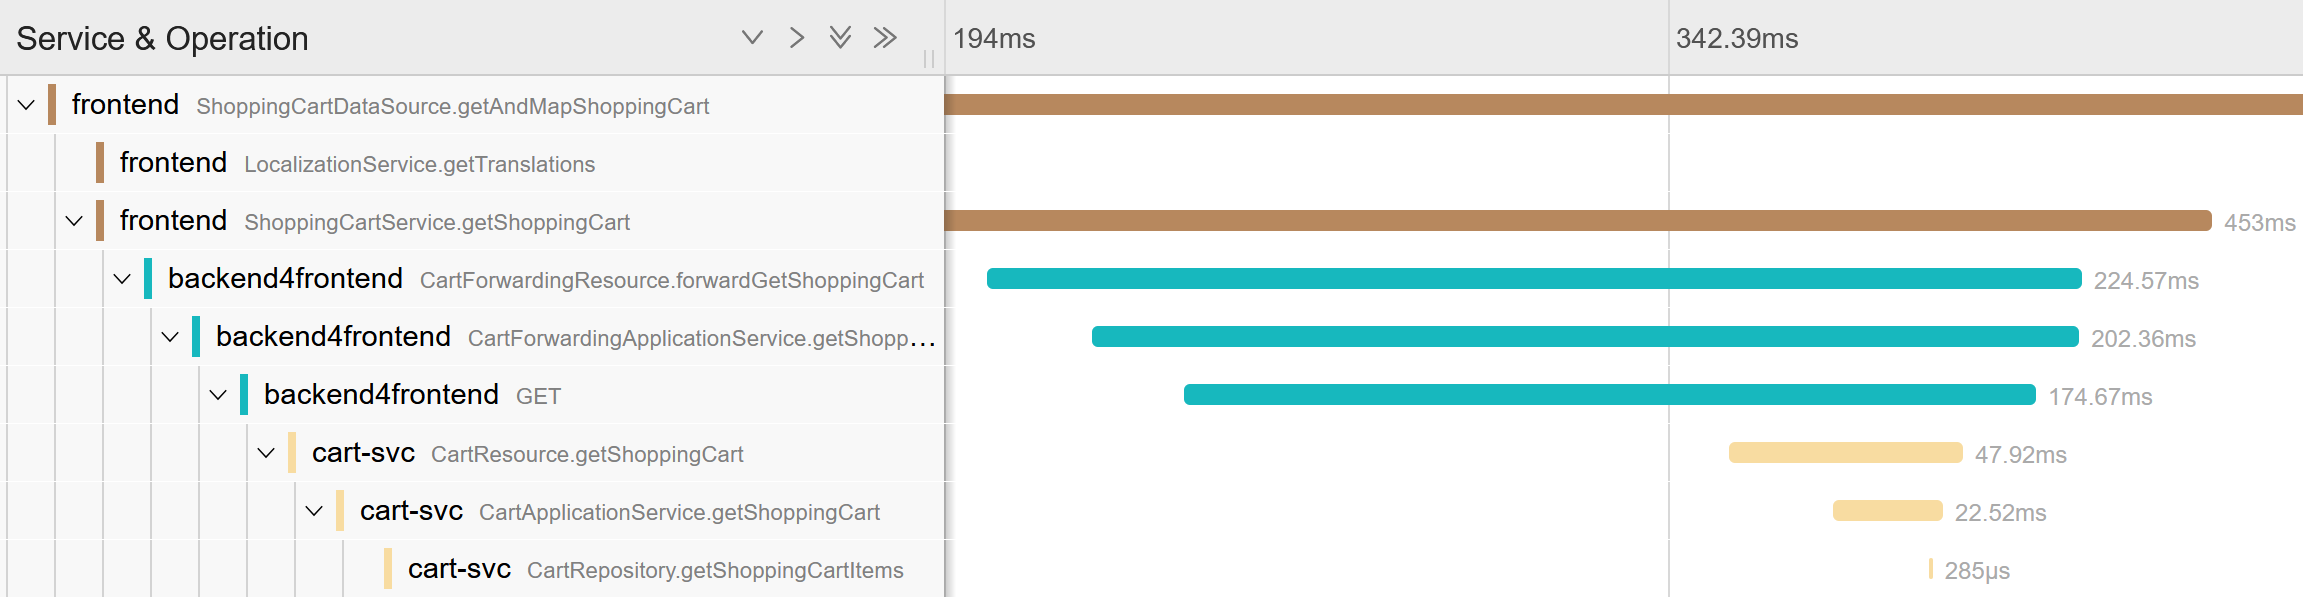
\includegraphics[width=\linewidth]{img/03_methoden/jaeger_trace-detail-view.png}
	\caption{Trace-Detailansicht. Eigener Screenshot aus Jaeger}
	\label{fig:jaeger-ui_trace-detail-view}
\end{figure}

\subsubsection{Sentry}
\label{subsec:sentry}

Sentry \cite{Sentry} ist ein SaaS-Produkt der Functional Software Inc., welches sich auf das Error-Monitoring spezialisiert. Die Kernfunktionalitäten beschränken sich auf das Error-Monitoring, auch wenn von anderen Praktiken einige Aspekte präsent sind, stellen diese keine eigens abgeschlossene Funktionalität dar.

Neben einer kommerziellen Version, stellt Sentry auch eine unbegrenzt kostenlos nutzbare Version bereit, welche im Rahmen dieser Arbeit evaluiert wurde. Der Quellcode für das Backend von Sentry ist, wie zuvor beschrieben, quelloffen verfügbar. Darüber hinaus wird zudem eine OnPremise-Lösung angeboten, die auf Docker basiert \cite{SentrySelfHosted}. Um von Webanwendungen Fehler zu erfassen und an Sentry zu melden, bietet Sentry bei NPM \cite{NPM} quelloffene Pakete an \cite{SentryJSGithub}. Dabei werden u. A. Anbindungen für folgende Technologien bzw. Frameworks bereitgestellt: JavaScript, Angular, React und Vue.js.

Wird ein Fehler gemeldet, erstellt Sentry hierzu ein \enquote{Issue}, also einen Problembericht. In einem Problembericht finden sich detaillierte Informationen zum Fehler, wie den Stacktrace, den Zeitstempel, die Nutzerumgebung (Browser, Version, etc.) sowie ein Ausschnitt der zuletzt aufgetretenen Logmeldungen in der Browserkonsole (vgl. \autoref{fig:sentry_issue-details}). Zudem schneidet Sentry jegliche Nutzerinteraktionen mit und stellt diese in dem Problembericht dar (vgl. \autoref{fig:sentry_issue-event-breadcrumbs}). Treten Fehler gleichen Ursprungs auf, fasst Sentry diese im selben Problembericht zusammen. Weiterhin kann jeder einzeln aufgetretener Fehler näher betrachtet werden.

Die angebotenen Fehlerinformationen von Sentry sind zahlreich und helfen beim Nachvollziehen besser als Logs und Traces allein. Eine ganzheitliche Nachvollziehbarkeit kann Sentry jedoch nicht anbieten, da die Informationen nur im Fehlerfall erhoben werden. Somit reicht Sentry nicht allein aus, um die in dieser Arbeit erwünschte Nachvollziehbarkeit zu erreichen.

\begin{figure}[H]
	\centering
	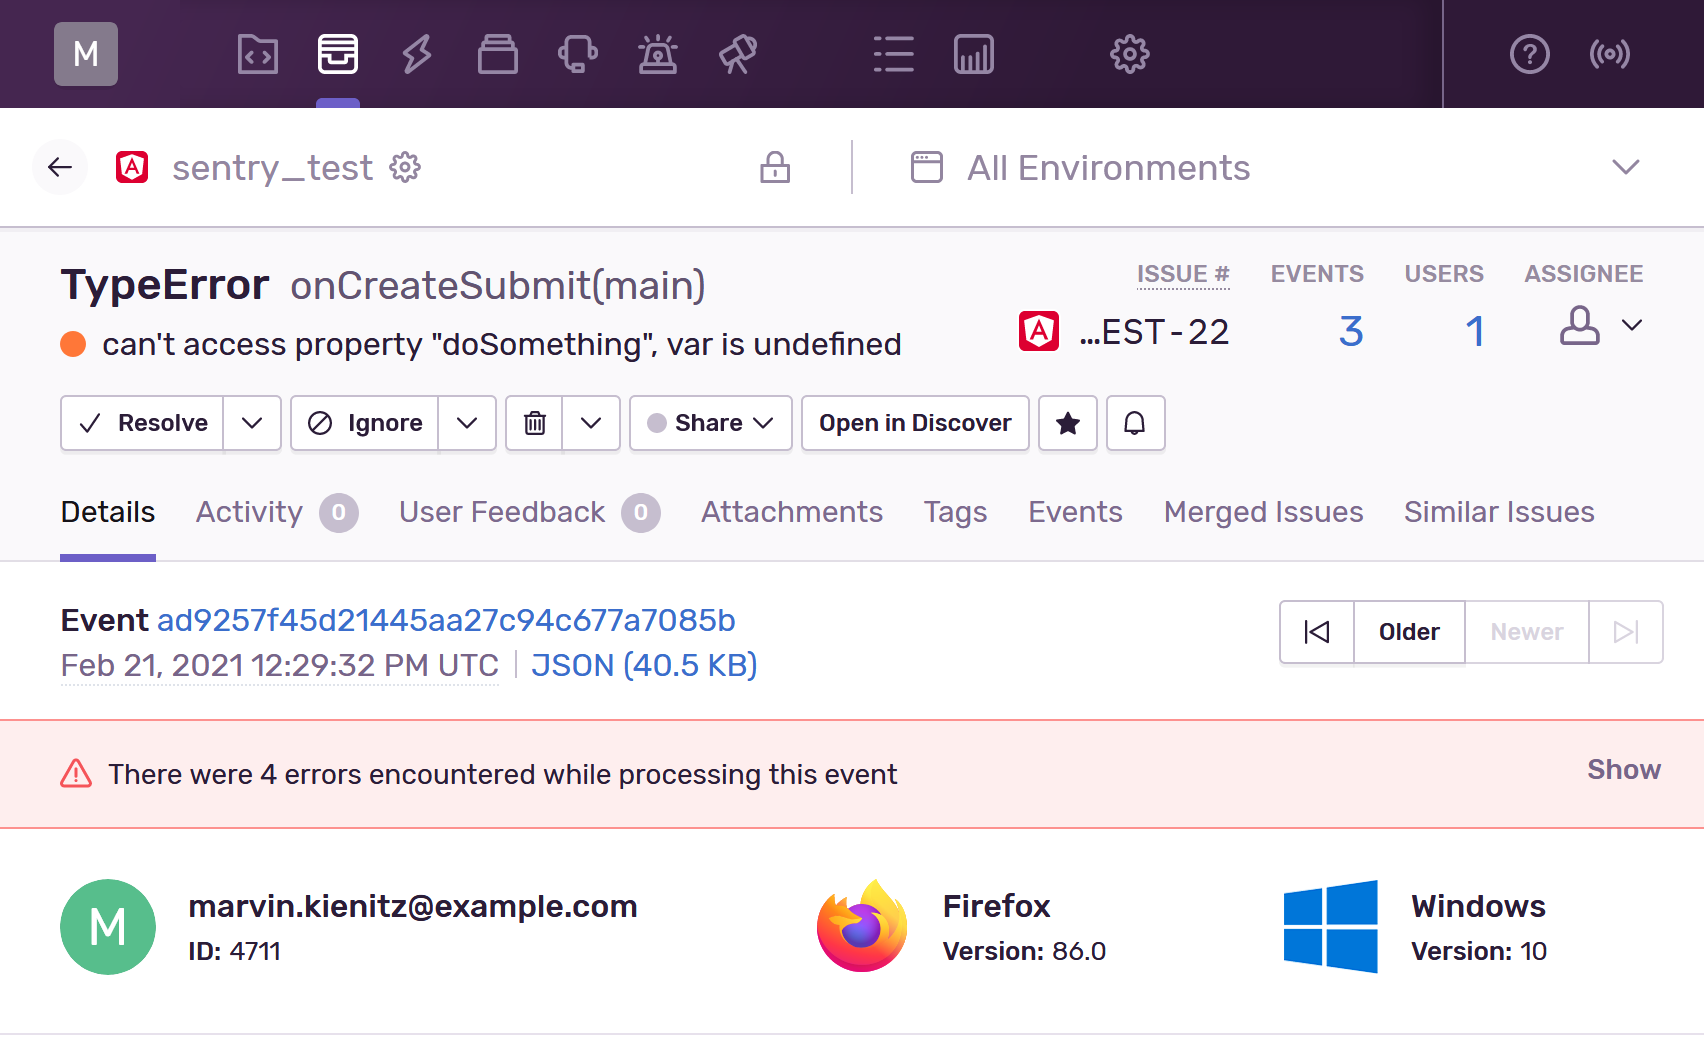
\includegraphics[width=1.00\linewidth]{img/03_methoden/sentry_issue-details.png}
	\caption{Kerninformation eines Issues. Eigener Screenshot aus Sentry}
	\label{fig:sentry_issue-details}
\end{figure}

\begin{figure}[H]
	\centering
	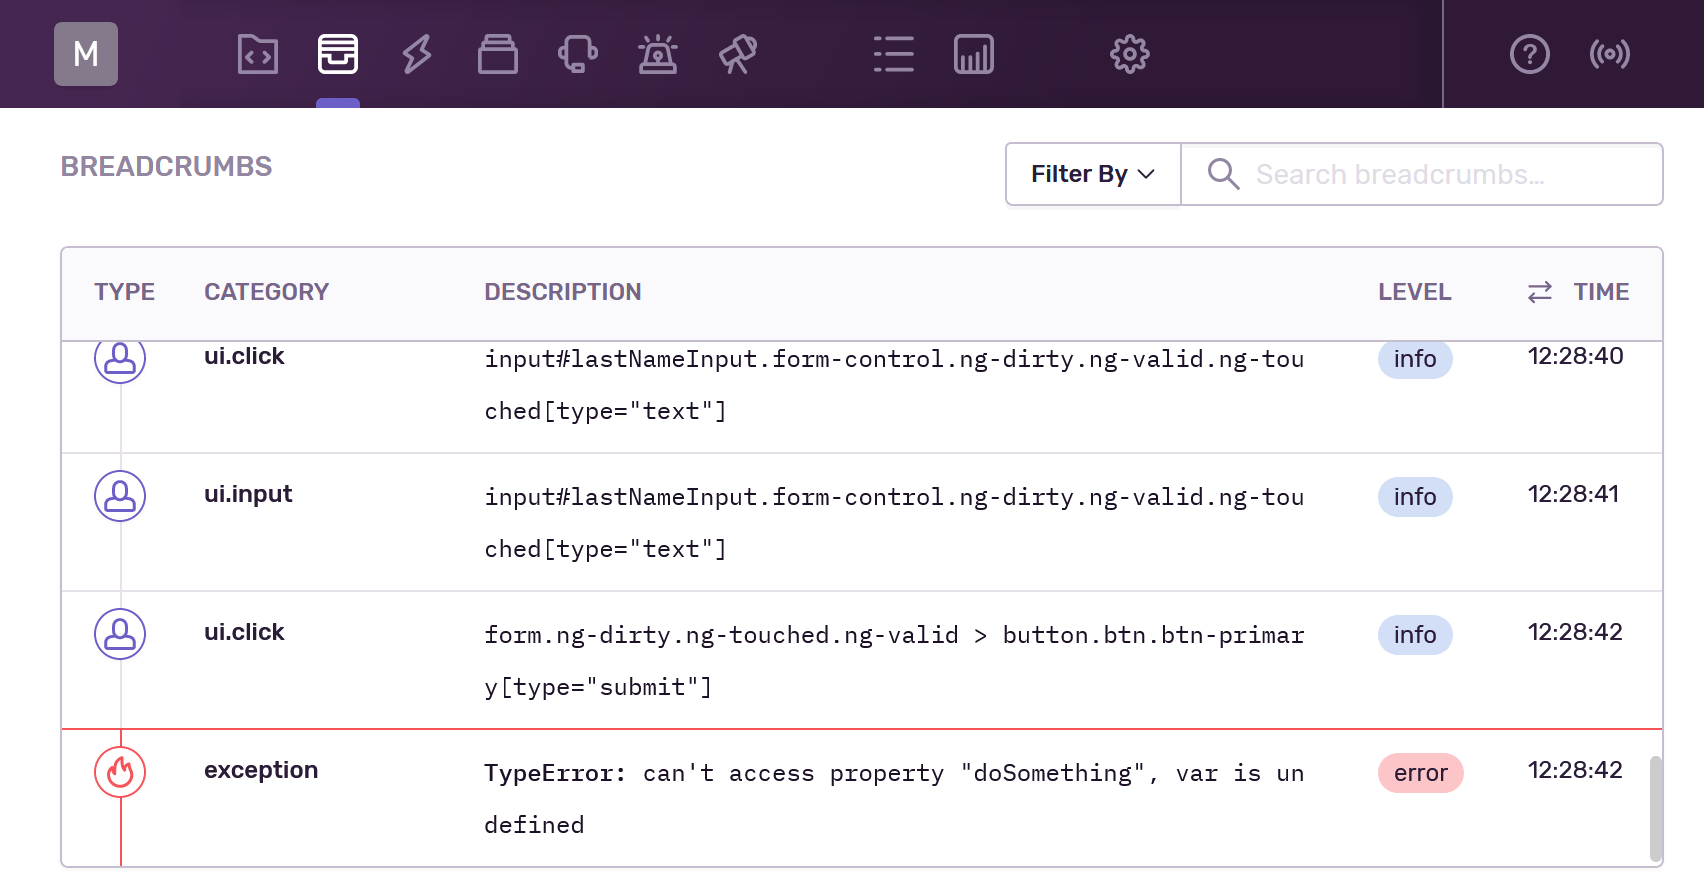
\includegraphics[width=1.00\linewidth]{img/03_methoden/sentry_issue-event-breadcrumbs.png}
	\caption{Verlauf der Userinteraktionen. Eigener Screenshot aus Sentry}
	\label{fig:sentry_issue-event-breadcrumbs}
\end{figure}

\subsubsection{LogRocket}
\label{subsec:logrocket}

LogRocket \cite{LogRocket} ist ein SaaS-Produkt des gleichnamigen Unternehmens und konzentriert sich auf detailliertes Session-Replay von JavaScript-basierten Clientanwendungen, um Probleme identifizieren, nachvollziehen und lösen zu können. Neben des SaaS-Produktes bietet LogRocket für Unternehmenskunden auch eine OnPremise-Lösung an. Anders als vergleichbare Session-Replay-Technologien nicht das Marketingteam o. Ä. \cite{Webalyt} die primäre Zielgruppe, sondern Entwickler.

LogRocket bietet eine kostenlose Testversion des SaaS-Produktes an, welche für die Evaluierung verwendet wurde. Zur Datenerhebung wird das Paket \texttt{logrocket} bei NPM \cite{NPM} angeboten, welches nach der Initialisierung eigenständig die notwendigen Daten sammelt. Mithilfe dieser Daten wird die gesamte Sitzung des Nutzers nachgestellt. Hierbei ist die Anwendung, die Nutzerinteraktionen, die Netzwerkaufrufe sowie das DOM zu sehen. Die Reproduktion wird videoähnlich aufbereitet und erlaubt ein präzises Nachvollziehen der zeitlichen Reihenfolge und Bedeutung (vgl. \autoref{fig:logrocket-session-replay-example}).

Neben dem JavaScript-SDK bietet LogRocket quelloffenene Plugins für folgende Bibliotheken: Redux, React, MobX, Vuex, ngrx, React Native. Zusätzlich bietet LogRocket auch eine Integration für andere Tools, wie z. B. Sentry. Bei der Integration für Sentry wird bei einem gemeldeten Fehler in Sentry direkt auf das \enquote{Video} in LogRocket verlinkt.

\begin{figure}[H]
	\centering
	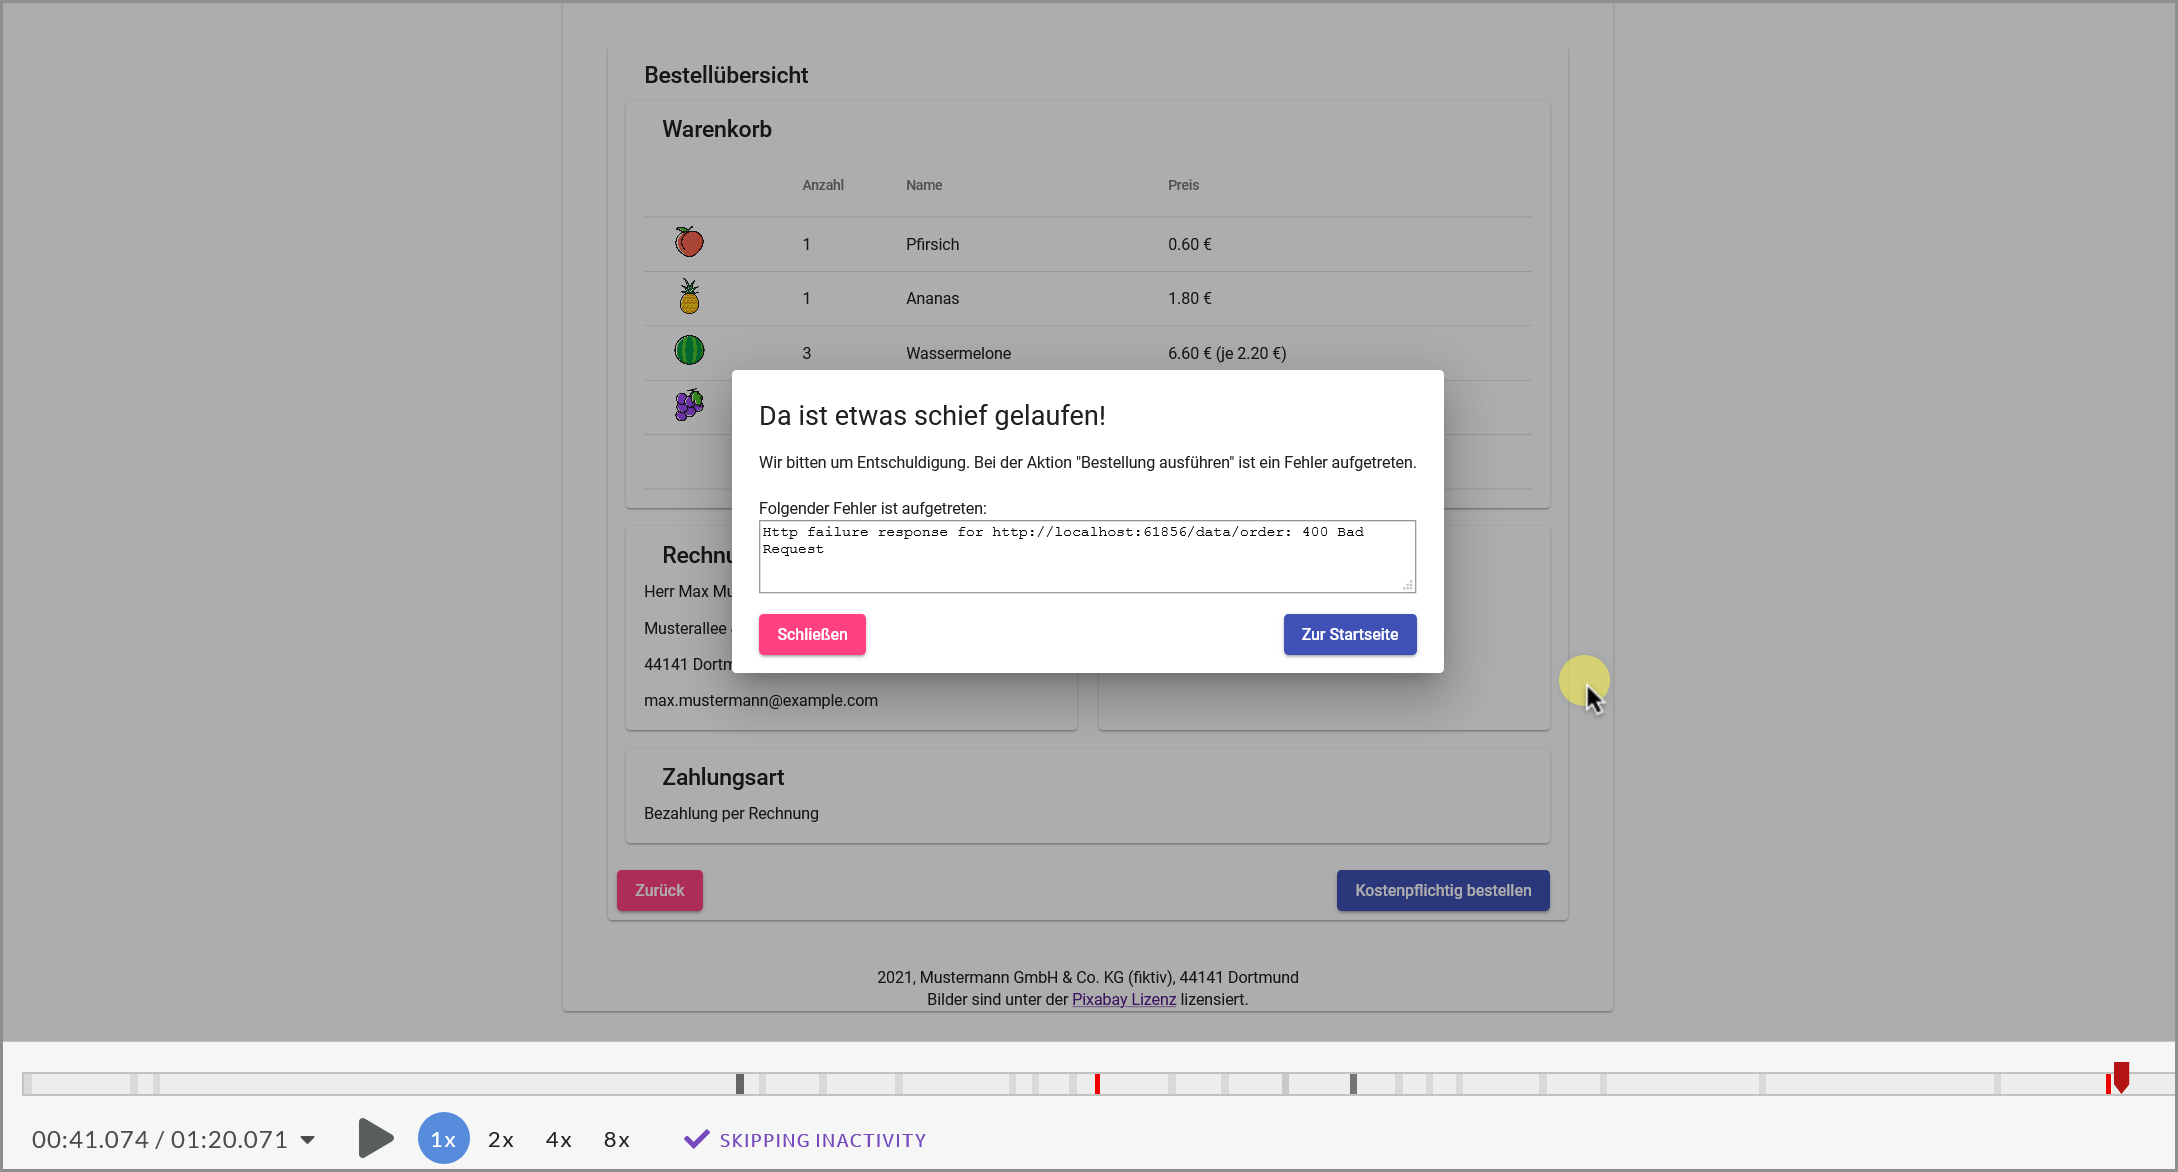
\includegraphics[width=\linewidth]{img/03_methoden/logrocket_session-replay-example-cropped.png}
	\caption{Ausschnitt eines Session-Replays. Eigener Screenshot aus LogRocket.}
	\label{fig:logrocket-session-replay-example}
\end{figure}